\documentclass[12pt]{article}
\usepackage{preamble}
\begin{document}

%%%%%%%%%%%%%%%%%frond page%%%%%%%%%%%%%%%%%%%%%%%%%%%%%%%%%%
\begin{titlepage}
\title{Firms' Carbon Emissions and Stock Returns}
\author{Giacomo Morelli\thanks{Department of Statistical Sciences, Sapienza University of Rome} \and 
Cong Wang\thanks{Department of Economics and Law, Sapienza University of Rome}}
\date{\today}
\maketitle
\begin{abstract}
\noindent In recent years, the surge of unanticipated climate change risk has propelled green assets to achieve superior returns compared to their brown counterparts. This contradicts the theoretical expectation that brown assets, exposed to higher risk compensations associated with climate change, should yield superior returns. This paper provides empirical evidence from the U.S. stock market, based on both portfolio and individual stock analysis. The results show that green portfolios characterized by lower carbon emissions consistently outperform their brown counterparts for the period from 2002 to 2020. Individual stock analysis shows similar results under different assumptions about the variations between or within industries. Notably, green assets exhibit higher returns, particularly during periods of heightened unexpected climate change concerns, aligning with the insights from \cite{ardia2022climate}..\\

\noindent\textbf{Keywords:} Carbon Emission, Stock Return, Climate Change\\

\noindent\textbf{JEL Codes:} G11, G12, G30\\
\bigskip
\end{abstract}
\setcounter{page}{0}
\thispagestyle{empty}
\end{titlepage}
\pagebreak \newpage

\doublespacing

%%%%%%%%%%%%%%%%%%%%%%%%%%%%%%%%%%%%%%%%%%%%%%%%%%%%%%%%%%%%%%%%
%%%%%%%%%%%%%%%%%%%%%%%%%%%%%%%%%%%%%%%%%%%%%%%%%%%%%%%%%%%%%%%%
\section{Introduction} \label{sec:introduction}
%%%%%%%%%%%%%%%%%%%%%%%%%%%%%%%%%%%%%%%%%%%

In the face of mounting challenges such as geopolitical conflicts, pandemics, and climate change, the call for sustainable investment and environmentally responsible production has never been more urgent. These pressing global concerns have underscored the critical need to prioritize sustainability as a central pillar of our collective future. In addressing these challenges, the United Nations, as outlined in \cite{fund2015sustainable}, has published Sustainable Development Goals (SDG) which comprises 17 interlinked objectives that emphasize the intricate connections between environmental, social, and economic aspects of sustainable development. Furthermore, the call for sustainable practices extends into the financial market, where sustainable investing has gained significant traction. Investors are increasingly recognizing the importance of integrating environmental, social, and governance (ESG) criteria into their decision-making processes as discussed in the report by \citet{BNPParibas2023}. In this context, the introduction of the Green minus Brown factor (GMB) in the current asset pricing literature, alongside established aggregate risk factors like small minus big (SMB), high minus low (HML), and robust minus weak (RMW), has emerged as a relevant factor explaining risks associated with climate change. Empirical evidence often shows that Green portfolios, in both stock and bond markets, outperform their Brown counterparts. However, classic asset pricing theories propose a contrasting view. These theories suggest that Brown assets, bearing greater risks associated with climate change, should offer higher returns as compensation for this increased risk. This presents a notable contradiction between empirical findings and theoretical predictions.

Investors frequently turn to ESG (Environmental, Social, and Governance) scores when evaluating companies to gauge their environmental, social and governance practices, especially the E scores for environment. These scores play an important role in categorizing companies into "Green" and "Brown", signifying their commitment to sustainable practices or their lack thereof. However, a notable challenge arises from the fact that multiple ESG rating agencies, such as MSCI ESG Ratings, Sustainalytics, and Bloomberg, among others, operate concurrently. Each of these agencies employs distinct valuation metrics and methodologies, leading to divergent ESG ratings for the same companies. In fact, recent research, as highlighted by \cite{avramov2022sustainable}, has revealed that this variation in ESG assessments can introduce uncertainty into the market. Such uncertainty has the potential to increase market premiums and diminish demand for the related stocks that exhibit higher ESG uncertainty, and create a complex landscape for investors to navigate. To circumvent the challenges associated with rating uncertainty, this paper adopts a pragmatic approach by relying on a single, yet robust, indicator to gauge companies' environmental performance: the Green House Gas (GHG) emissions. GHG emissions are recognized as a primary driver of global warming, and they are mandated for disclosure by various stakeholders, including the Securities and Exchange Commission (SEC), investors, and the public media. By focusing on this widely accepted and easily measurable metric, this study seeks to provide a clear and unambiguous assessment of firms' sustainability practice and their stock returns. 

Our analysis investigates whether firms characterized as "Brown" due to their higher carbon emissions experience higher stock returns compared to "Green" firms, as posited by classic theoretical studies suggesting that higher risk exposure is associated with higher returns. This analysis focuses exclusively on the U.S. stock market. The dataset utilized in this study encompasses all publicly traded stocks in the U.S. stock market from 2002 to 2021. The initial step of this research involves an exploratory analysis of the relationship between firms' carbon emissions and their stock returns cross-sectionally. For the entire dataset, we categorize all the observations into percentiles based on total CO2 emissions, subsequently computing the average stock return within each percentile. The findings reveal that stocks situated in the lower percentiles consistently exhibit higher average stock returns, with a decline in returns observed as percentiles progress toward the 100th percentile. Remarkably, this pattern persists when we consider different scopes of carbon emissions. It's worth noting that while one might attribute this trend to other firm characteristics such as size, as carbon emissions tend to be positively correlated with firm size, our analysis does not reveal a similar pattern between firm size and stock returns, as well as other factors such as leverage, profitability, and growth. Furthermore, we apply a similar methodology to examine the relationship between firms' stock returns and carbon intensity, defined as a firm's carbon emissions scaled by its revenue. This matric is a crucial proxy for a firm's carbon footprint in the current corporate finance literature. However, in contrast to our findings on carbon emissions, we do not identify a clear and consistent relationship between firms' stock returns and carbon intensity.

Is it, however, conclusive to assert that firms with lower carbon emissions consistently yield higher stock returns? Not necessarily, as there is significant heterogeneity in carbon emissions across different industries. For instance, the Power and Renewable Electricity sector\footnote{The industry classification in this paper follows the Global Industry Classification Standards (GICS).} leads with an average emission of 38.15 million tons annually, a stark contrast to the Mortgage Real Estate Investment Trusts (REITs) 0.03 million tons. This disparity makes a direct comparison among firms belonging to different industries akin to contrasting apples with bananas. To address this, we conduct a more nuanced analysis. Stocks within each industry are divided into quintiles based on their carbon emissions. Within each industry, we then create value-weighted portfolios: 'Green' for stocks with the lowest emissions, 'Brown' for the highest, and 'Neutral'\footnote{Here the carbon neutral portfolios do not mean that the underlying companies have zero carbon emission, but these companies are ranked in the middle tertiles in the industry with respect to carbon emission.} for the middle range\footnote{The second and fourth quintiles are excluded from our analysis for a more distinguish comparison between firms in different range of carbon emissions.}. Over the entire dataset spanning from 2002 to 2021, the Green portfolios have delivered impressive cumulative returns, exceeding 600\%, while their Brown counterparts achieved approximately 270\% in cumulative returns, the result coincides with \cite{pastor2022dissecting} who use ESG scores to construct Green and Brown portfolios. However, when we replicate this approach using firms' carbon intensity, the results diverge. The outperformance of green portfolios is not as clear as before, and it is only observed after 2010.

Through a comprehensive regression analysis, we unearth intriguing insights into the performance of Green and Brown portfolios based on different criteria. When considering firms' total carbon emissions, Green portfolios exhibit a statistically significant monthly outperformance of 44.3 basis points over their Brown counterparts. However, when evaluating portfolios constructed based on carbon intensity, the difference between Green and Brown portfolios narrows to a mere 0.4 basis points, with no statistical significance observed. Delving deeper into the analysis, we apply the Fama-French 5 factors model to regress the GMB (green minus brown) portfolios. An intriguing finding emerges in the form of a significant intercept that defies explanation, suggesting the presence of an unaccounted factor, possibly the Green minus Brown factor discussed by \cite{pastor2022dissecting}. 

Another paper by \cite{pastor2021sustainable} posits that Green portfolios outperform Brown in the presence of unexpected climate change-related concerns. To further illuminate this relationship, we leverage the Media Climate Change Concern (MCCC) index developed by \cite{ardia2022climate} and employ an ARX model to compute the Unexpected Media Climate Change Concerns (UMC) just like the authors do in their study. The regression results reveal a positive relationship between UMC and GMB portfolios. Specifically, a 1-unit increase in UMC index corresponds to a 1.49\% increase in the return of GMB portfolios, with statistical significance observed at the 1\% level. Moreover, when we conduct separate regressions of the UMC index on Green and Brown portfolios, distinct patterns emerge. The coefficient on Brown portfolios stands at -1.27, signifying that in periods of elevated unexpected climate risk, the return for Brown portfolios experiences a notable decline. In contrast, the coefficient of the UMC index on Green portfolios is positive at 0.23, indicating that a higher UMC index is associated with higher returns for Green portfolios. Remarkably, the UMC index does not exhibit statistical significance concerning the return of Neutral portfolios, highlighting the selective impact of unexpected climate concerns on the investment performance of different portfolios.

In our aggregated portfolio analysis, our findings align with \cite{pastor2022dissecting}, suggesting that Green portfolios, which encompass firms with higher ESG scores or lower carbon emissions, tend to outperform their Brown counterparts. These results are corroborated by \cite{friede2015esg}, who also indicate that Green firms often exhibit better financial performance. However, when we delve into firm-level analyses, as conducted by \cite{bolton2021investors} and \cite{aswani2023carbon}, a stark contradiction emerges. Their research suggests that firms with higher carbon emissions tend to yield higher stock returns, directly conflicting with our portfolio performance findings.

To address this discrepancy, we shift our focus to firm-level data and employ panel Ordinary Least Squares (OLS) regression to explore the relationship between firms' total carbon emissions and stock returns. Recognizing the presence of unobserved time-variant factors and time-invariant industry-specific factors, we incorporate Industry + Time fixed effects in our panel regression model. Our results reveal a positive correlation between firms' stock returns and total carbon emissions indicating that firms with higher CO2 emissions tend to have higher stock returns on average, yet this relationship lacks statistical significance. 

The choice to incorporate Industry + Time two-way fixed effects is rooted in the assumption that there exist unobserved time-variant factors associated with time periods and time-invariant factors linked to industries. This assumption hinges on the belief that firms within the same industry during the same time period exhibit similar stock return behaviors. A more stringent assumption is that even in the same industry firms' stock returns still behave differently, due to some idiosyncratic characteristics associated with each specific firm. Under this new assumption, we apply Entity + Time two-way fixed effects. The results of this analysis reveal a significant and negative relationship between firms' carbon emissions and stock returns, both statistically and economically. Specifically, a 1\% increase in firms' total carbon emissions corresponds to a 0.66\% decrease in stock returns, on average. These findings provide robust support for the notion that higher carbon emissions are associated with lower stock returns alongside our portfolio analysis, emphasizing the importance of accounting for idiosyncratic firm-level characteristics in our analysis. In our robustness analysis, we systematically vary the fixed effects and cluster standard errors at different levels. Notably, whenever we incorporate entity-fixed effects into the model, our findings consistently align with those of our benchmark model. This robustness underscores the reliability and stability of our results across various specifications, affirming the significance of entity-fixed effects in our analysis

In line with \cite{pastor2021sustainable}, who developed an equilibrium model based on ESG scores and stock returns, our firm-level analysis delves into the relationship between firms' carbon emissions, unexpected climate change concerns, and stock returns. We find that when unexpected climate change concerns materialize, brown firms characterized by higher total CO2 emissions tend to experience decreases in their stock returns. Importantly, these results hold true across various sets of control variables containing macroeconomic conditions. After accounting for factors such as the Fama-French 5 factors, the investor sentiment index, the CFNAI index, WTI, and VIX, the interaction between firms' total carbon emissions and unexpected climate concerns remains significant, demonstrating a negative impact on stock returns, and the statistical significance is observed at the 1\% level. This robustness reinforces the link between firms' carbon emissions and stock performance in the face of climate change concerns. When unexpected climate change concerns hit the economy, firms with higher carbon emissions (Brown Firms) experience losses in their stock returns. 

\subsection*{Related Literature}

Our study contributes to a vast empirical literature on sustainable investing, encompassing both aggregated portfolio and firm-level analyses. In a broader context, research in this field has gained significant momentum due to growing concerns about climate change and sustainability. For instance, \cite{krueger2020importance} conducted a study using survey data to investigate climate perception and found that climate risks, particularly those related to regulations, have started to materialize. Their research indicates that many investors, particularly those with a long-term perspective, larger portfolios, and a focus on ESG (Environmental, Social, and Governance) factors, prioritize risk management and engagement over divestment strategies. This underscores the evolving priorities and strategies of investors in response to climate-related challenges. 

Similarly, \cite{faccini2023dissecting} conducted groundbreaking research to assess whether market-wide physical or transition climate risks are priced into U.S. stocks. They found that only the climate-policy factor is priced, especially after 2012. Interestingly, their study revealed that investors seem to be less concerned about natural disasters, global warming, and decisions made at international climate summits. This research highlights the complexity of integrating climate risk into financial markets and the selective focus of investors on specific aspects of climate-related factors. 
		
In the midst of this dynamic landscape, our study adds to the body of knowledge by examining the relationship between firms' carbon emissions, climate change concerns, and stock returns. However, the current literature diverges when it comes to the performance of Green and Brown assets.  \cite{garvey2018carbon} have utilized carbon ratios to select stocks, revealing that lower carbon ratios are associated with higher stock returns and increased profitability. \cite{in2017being} constructed "Efficient-Minus-Inefficient" portfolios based on carbon intensity, demonstrating their ability to generate positive alpha since 2009. Meanwhile, \cite{andersson2016hedging} introduced a low carbon index, and find that when climate change mitigation is pending, the low carbon index performs the same as the benchmark, when carbon emission is priced, the index outperforms the benchmark. Additionally, \cite{hsu2023pollution} investigated the impact of toxic emissions intensity within industries, showcasing that the portfolio premium could not be explained by traditional factors, sentiment, political connections, or corporate governance, emphasizing the unique role of toxic emissions in stock returns. These studies all suggest that Green assets characterized by lower carbon emissions generate climate risk premiums, and outperform Brown assets especially when there are emission-related policy shocks.

Another branch of study declares that investors are already demanding compensation for carbon emission risk, hence Brown assets are associated with higher expected returns. Notably, studies like \cite{bolton2021investors} and \cite{aswani2023carbon} have found that firms with high CO2 emissions tend to yield higher stock returns, showcasing the influence of carbon intensity on investment choices for institutional investors, particularly in salient industries. \cite{baker2018financing} delved into the world of green bonds, which are used for environmentally sensitive purposes, and identified that green bonds are issued at a premium compared to otherwise similar ordinary bonds, highlighting investor demand for environmentally responsible investments. Meanwhile, \cite{zerbib2022sustainable} introduced the concept of exclusion premia, encompassing sin stocks, to elucidate the relationship between ESG factors and financial performance. They found that exclusion effects amounted to 2.79\% annually, with taste effects varying from -1.12\% to 0.14\%. Moreover, \cite{chava2014environmental} analyzed the impact of a firm's environmental profile on its cost of equity and debt capital, discovering that investors demanded significantly higher expected returns on stocks excluded by environmental screens compared to firms without such concerns. These excluded firms also exhibited lower institutional ownership and fewer banks participating in their loan syndicates. Additionally, \cite{bolton2021global} estimated the market-based premium associated with carbon risk at the firm level across 77 countries, uncovering a widespread carbon premium characterized by higher stock returns for companies with higher levels of carbon emissions. Lastly, \cite{gorgen2020carbon} found that Brown firms tended to yield higher average returns, while decreases in the greenness of firms were associated with lower announcement returns. However, when they constructed a carbon risk factor-mimicking portfolio, they did not find evidence of a carbon risk premium, emphasizing the complexity of the relationship between carbon risk and investment returns.

In response to the significant divergence between two contradictory branches of existing literature, this study adopts a comprehensive approach encompassing aggregated portfolio analysis and firm-level investigations. By bridging the gap and synthesizing findings from both approaches, we aim to provide a more holistic and nuanced understanding of the relationship between stocks' greenness, measured by their carbon emissions, and their corresponding stock returns.

%%%%%%%%%%%%%%%%%%%%%%%%%%%%%%%%%%%%%%%%%%%%%%%%%%%%%%%%%%%%%%%%
%%%%%%%%%%%%%%%%%%%%%%%%%%%%%%%%%%%%%%%%%%%%%%%%%%%%%%%%%%%%%%%%
%\section{Literature Review} \label{sec:literature review}
%\input{2. Literature review}
%\clearpage
%%%%%%%%%%%%%%%%%%%%%%%%%%%%%%%%%%%%%%%%%%%%%%%%%%%%%%%%%%%%%%%%
%%%%%%%%%%%%%%%%%%%%%%%%%%%%%%%%%%%%%%%%%%%%%%%%%%%%%%%%%%%%%%%%
\section{Methodology} \label{sec:Methodology}
%\input{3. Methodology}
The current literature presents seemingly contradictory findings regarding the relationship between a firm's environmental practices and its stock performance. Conventional theoretical studies typically associate higher risk exposure with increased return compensation. \citet{bolton2021investors} use firm-level data and find a positive correlation between a firm's carbon emissions and its stock returns, indicating that brown assets outperform green ones. They argue that investors demand higher returns as compensation for climate-related risks aligning with the theoretical perspectives. In contrast, \cite{pastor2021sustainable} develop a new theoretical model suggesting that environmentally friendly assets typically yield higher returns, particularly in the face of unexpected climate change concerns. This model is further supported by empirical evidence from \cite{pastor2022dissecting}, who find that in the U.S. stock market, portfolios with higher Environmental, Social, and Governance (ESG) scores (Green portfolios) outperform those with lower ESG scores (Brown portfolios). A similar trend is observed with German green bonds outperforming their brown counterparts. This paper aims to reconcile these seemingly contradictory findings from existing literature. The methodologies used in this empirical study are introduced in this section.

\subsection{Quantify Firms' Environmental Practices}

In the current research, two primary methodologies are employed to quantify firms' environmental practices. The first one involves utilizing Environmental, Social, and Governance (ESG) scores provided by third-party rating agencies, such as Bloomberg, Thomson Reuters, MSCI ESG Ratings, and Sustainalytics. However, the diversity of rating agencies and their differing methodologies often lead to variations in the final ESG scores for the same company. This inconsistency can introduce what is known as ESG uncertainty. \cite{avramov2022sustainable} demonstrate that this ESG uncertainty can result in increased CAPM alpha and effective beta, as well as investment outflows from stocks exhibiting high ESG uncertainty. Additionally, ESG scores are susceptible to influences that may not directly relate to a firm's environmental performance. For instance, larger corporations often have greater resources for managing their public image and ESG reporting, potentially resulting in inflated scores (known as 'greenwash') that may not accurately reflect their environmental practices, especially in comparison to smaller companies.

The second methodology for quantifying firms' environmental practices involves direct measurements of specific environmental metrics, such as carbon emissions, water usage, and waste production. This method offers a more objective and quantifiable approach, independent of the subjective assessments of third-party ESG ratings. In this paper, following the precedent set by \cite{bolton2021investors} and \cite{ardia2022climate}, we focus on carbon emissions as a key metric for assessing firms' environmental practices. Carbon emissions are a significant contributor to climate change and their reporting has become increasingly mandated by regulatory bodies in recent years, providing a more consistent and standardized data set for analysis. Additionally, this paper considers carbon intensity - a metric that relates a firm's carbon emissions to its revenue. Carbon intensity measures the efficiency with which a firm generates revenue relative to the Greenhouse Gases (GHG) it emits, as highlighted by \cite{ilhan2021carbon}. 

\subsection{Aggregate Portfolio Analysis}
Comparing CO2 emissions directly across companies from different industries can be misleading due to their unique operational requirements and regulatory environments inherent to different industries. For instance, the high emissions in the energy sector, particularly from fossil fuels, cannot be directly compared with the lower emissions of the technology or service sectors. Therefore, in this paper we take a more accurate assessment by comparing emissions within the same industry, allowing for fair benchmarking against industry-specific standards and regulations. This approach highlights companies leading in sustainability and green practices relative to their peers and it could provides a realistic view of each company's efforts to reduce emissions. It can be expressed in the following equation:

\begin{equation}
\label{eqn: measure greenness}
Greenness_{i, t} = \mathbb{E}[Greenness_{i,t} | CO2 \: Emissions_{i, t}, Industry_i]
\end{equation}

In Equation \ref{eqn: measure greenness}, we measure company $i$'s sustainable practices at time $t$ within industry, based on its carbon emission. Essentially, this method accounts for the heterogeneity between industries, offering a more nuanced understanding of environmental impacts and sustainability efforts. Utilizing this methods, we categorize stocks into quintiles at a monthly basis and create value weighted portfolios for each quintiles. Stocks in the lowest quintile construct "Green" portfolio characterized by low carbon emission. Conversely, portfolios formulated by stocks from the top and middile quintiles are defined as "Brown" and "Netural", respectively. We also build a "Green-Brown" portfolios by long the lowest deciles and short the top deciles aligning with \citet{pastor2022dissecting} and \citet{ardia2022climate}.

In their equilibrium model, \citet{pastor2021sustainable} propose that green assets typically yield lower expected returns than brown assets for two reasons: investors' preference for green investments and the superior ability of greener assets to hedge against climate risk. These lower expected returns are attributed to both a taste premium and a risk premium. However, the model also suggests that green assets can exhibit higher realized returns when there is an unexpected shift in investor demand towards greener options. To empirically test this theoretical framework, we employ a multivariate linear regression model that controls for other factors influencing stock returns. We specifically regress the returns of "Green-Brown," "Green," "Brown," and "Neutral" portfolios against the Unexpected Media Climate Change Concerns ($UMC_t$), as constructed by \citet{ardia2022climate}.

\begin{equation}
\label{eqn: regression portfolio}
RET_{p, t} = \alpha_p + \beta^{UMC}_{p}*UMC_t + \beta^{contr}_p*Controls_t + \epsilon_{p, t}
\end{equation}

\noindent In the model, $RET_{p, t}$ represent the return of portfolio $p$, at time $t$. The intercept is denoted as $\alpha_p$, while $\beta^{UMC}_p$ is the coefficient for $UMC$ index, $\beta^{contr}_p$ presents a vector of coefficients corresponding to a series of control factors, and $\epsilon$ is the idiosyncratic error term. The $UMC_t$ index quantifies unexpected media climate change concerns, derived from news about climate change in widely circulated U.S. newspapers. An increase in this index suggests heightened concerns about climate change, which is expected to trigger a shift in investor preferences towards green assets.

\subsection{Individual Stock Analysis}
For the analysis of individual stocks, we directly examine the relationship between a firm's carbon emissions and its stock returns. We utilize the two-way fixed effects (TWFE) panel regression in our benchmark regression to investigate this relationship. The specific regression model, denoted as \ref{eqn: firm_base}, assesses the impact of carbon emissions on stock returns:

\begin{align}
    \label{eqn: firm_base}
    RET_{i, t} &= \alpha + \beta^{co2}*\log(co2 \: emission_{i, t}) + \beta^{contr}*Controls_{i, t} + \epsilon_{i, t}
\end{align}
    
Here, the subscript $i$ refers to company $i$, and $t$ indicates a specific month. $RET_{i, t}$ represents the return of stock $i$ in month $t$. The term $\alpha$ is the cross-sectional intercept, while $\beta^{co2}$ is the coefficient on firms' carbon emissions. The logarithmic normalized carbon emissions are expressed as $\log(co2 \: emission)$. The vector $\beta^{contr}$ comprises coefficients for a series of control variables. Industry and time fixed effects are incorporated through $Industry_{i}$ and $Time_{t}$, respectively, aligning with the methodology of \citet{bolton2021investors}. Lastly, $\epsilon_{i, t}$ denotes the idiosyncratic error term. The parameter of interest is $\beta^{co2}$, which presents the relationship between carbon emissions and firms' stock returns. A significant positive $\beta^{co2}$ demonstrantes empirical evidence that higher carbon emission associate higher stock return which algin with the classic asset pricing framework that higher risk exposure associate with higher return compensation.

Similar to our aggregate portfolio analysis, it is equally interesting to investigate the impact of $UMC$ at the individual stock level, particularly how the interaction between a firm's carbon emissions and $UMC$ influences the firm's stock returns. To assess this, we employ a firm fixed-effect panel regression model as follows:

\begin{align}
    \label{eqn: firm_interaction}
    RET_{i, t} &= \alpha + \beta^{co2}*\log(co2 \: emission_{i, t}) + \beta^{umc}*UMC \nonumber \\
               &\quad + \beta^* *(log(co2 \: emission_{i, t})*UMC_{t}) \nonumber \\
               &\quad + \beta^{contr}*Controls_{i, t} + \epsilon_{i, t}
\end{align}

\noindent Different from Equation \ref{eqn: firm_base}, we include $UMC_{t}$ and the interaction between $log(co2 \: emission_{i, t})$ and $UMC_t$ in Equation \ref{eqn: firm_interaction}. The key coefficient, $\beta^*$, is of particular interest as it determines whether $UMC$ amplifies or diminishes the link between a firm's carbon emissions and its stock return. The relationship is detailed in Equation \ref{eqn: derivation}. If $\beta^{co2}$ and $\beta^{umc}$ are both positive, high unexpected climate change concerns could lead to even higher returns for brown stocks to compensate for increased risk exposure. Conversely, if $\beta^{co2}$ and $\beta^{umc}$ both have negative signs, the green stocks will realize even higher returns. If $\beta^{co2}$and $\beta^{umc}$ have opposite signs, the impact of unexpected climate change concerns on the relationship between carbon emissions and stock returns could be mitigated.

\begin{equation}
\label{eqn: derivation}
\frac{\partial RET{i, t}}{\partial log(co2 \: emission_{i, t})} = \beta^{co2} + \beta^{umc}*UMC_{t}
\end{equation}
%%%%%%%%%%%%%%%%%%%%%%%%%%%%%%%%%%%%%%%%%%%%%%%%%%%%%%%%%%%%%%%%
%%%%%%%%%%%%%%%%%%%%%%%%%%%%%%%%%%%%%%%%%%%%%%%%%%%%%%%%%%%%%%%%
\section{Data} \label{sec: data}
%%%%%%%%%%%%%%%%%%%%%%%%%%%%%%%%%%%%%%%%%%%%%%%%%%%

This study exclusively examines publicly traded companies in the U.S. stock market from 2002 to 2021. Our dataset merges carbon emission data from Trucost, financial accounting information from Compustat, and stock return figures from CRSP (The Center for Research in Security Prices), with the CUSIP-PERMNO linkage table serving as the connector. Trucost's dataset offers insights into the environmental impacts of various business activities and evaluates risks associated with a wide array of environmental issues. These include carbon and other pollutants, water dependency, natural resource efficiency, and waste management. The data from Trucost includes both raw and calculated values at both the company and sector levels. Following the approach of \citet{aswani2023carbon}, we opt for the calculated carbon emission data, considering its comprehensiveness and relevance to stock returns. The merged dataset comprises 5,250 companies, totaling 526,393 observations. As illustrated in Figure \ref{fig: num}, the graph displays the annual count of both companies and observations. Notably, the carbon emission data collection began in 2002 with limited coverage. However, since 2016, there was a substantial surge in the number of companies included in the dataset, for the coverage for samll- amd mid-cap companies starts from 2016. This remarkable expansion algin with the assignement of various international agreements during this period, such as the \textit{Addis Ababa Action Agenda} (AAAA), the \textit{Sendai Framework for Disaster Risk Reduction 2015-2030} (SFDRR), and \textit{The Paris Agreement on Climate Change}. These agreements, as discussed by \cite{engberg2021influence}, \cite{kelman2015climate}, and \cite{dimitrov2016paris}, have played an important role in addressing global climate challenges, emphasizing the importance of sustainable development and initiatives targeting climate change.

\begin{figure}[!ht]
\centering
\caption{\textbf{Number of Firms and Observations}}
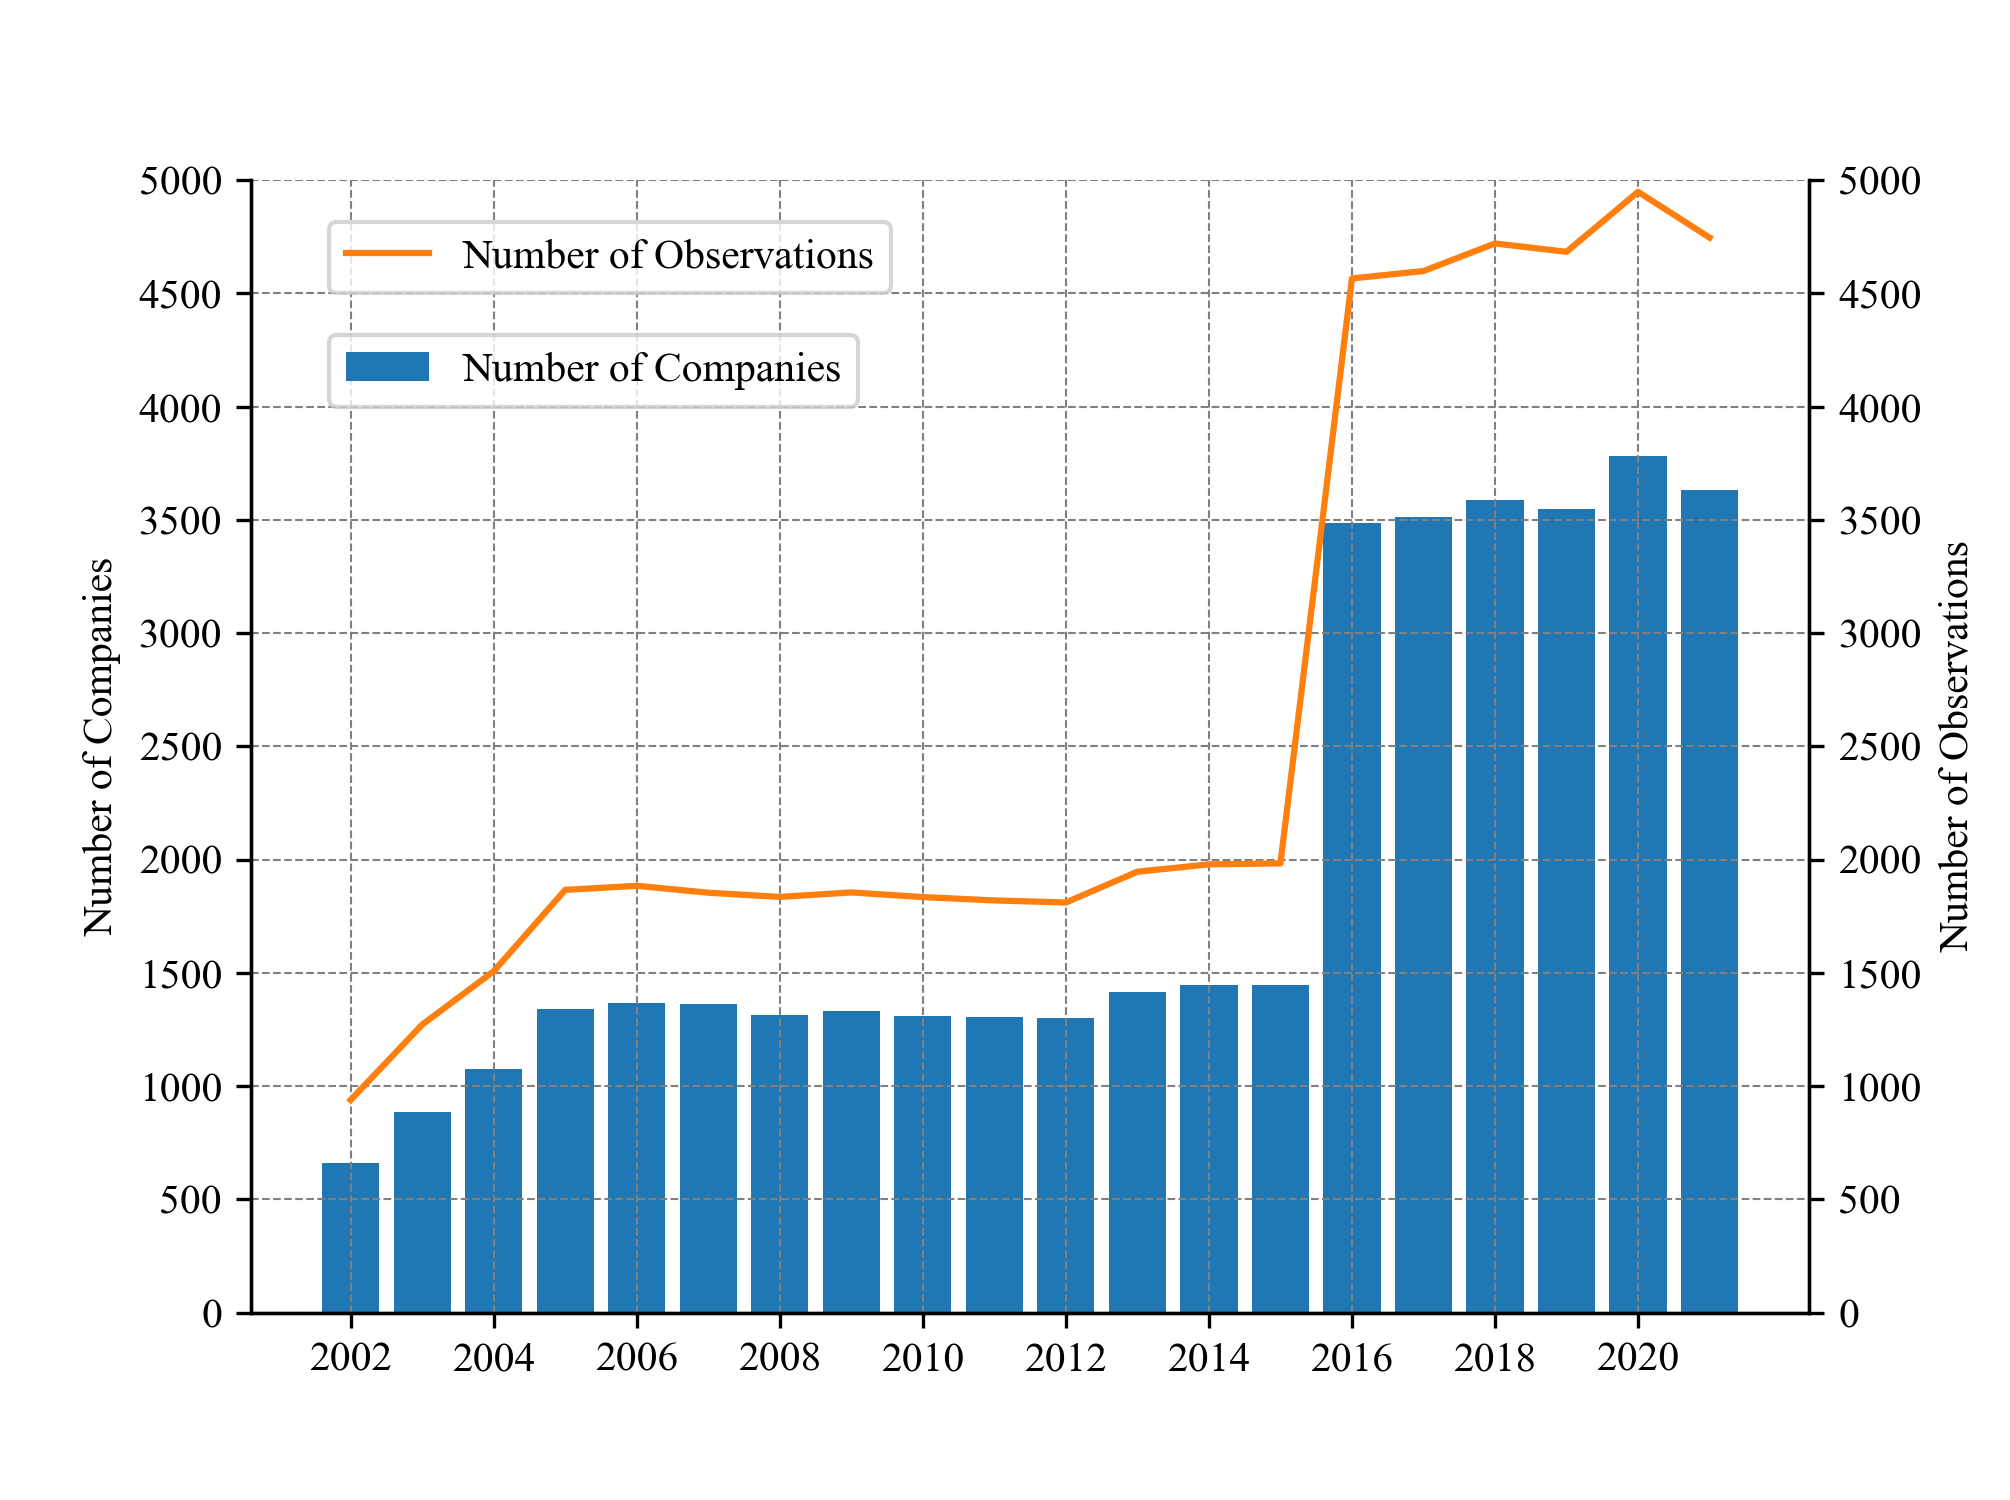
\includegraphics{graphics/number_obs.png}
\label{fig: num}
\caption*{\footnotesize{This graphic plots the number of firms and observations across the whole sample period.}}
\end{figure}

%%%%%%%%%%%%%%%%%%%%%%%%%%%%%%%%%%%%%%%%%%%%%%%%%%%
\subsection{Variable definition and summary statistics}

We provide explanations for key variables outlined in Table \ref{tab: var def}. The stock return data incorporates stocks' capital gains and dividends, observed monthly. The companies' total carbon emission data is the sum of all 3 scopes of emissions collected by Trucost follwo the Greenhouse Gas Protocol: Scope 1 entails direct greenhouse gas emissions, Scope 2 covers indirect emissions from purchased energy consumption, and Scope 3 encompasses a wider range of upstream and downstream indirect emissions. While, carbon intensity is calculated as the ratio of carbon emissions to revenue (tons/million(USD)), indicating how effectively a company utilizes its CO2 emissions to generate revenue. Control variables in this analysis encapsulate fundamental financial conditions, which have been substantiated as pertinent factors influencing stock returns through extensive literature such as \cite{perez2000firm}, \cite{george2010resolution}, and \cite{lamont2000investment}. The size is a firm's market capitalization in logarithmic form, serving as a measure of its economic scale; leverage, which quantifies a firm's financial structure risk by assessing the ratio of total liability to market capitalization; B/M (Book-to-Market Ratio) indicating the difference between firms' book value and market valuation; RoE (Return on Equity) capturing firms' profitability through the return generated on shareholders' equity; Invest/AT (Investment to Total Assets) reflecting firms' innovation efforts by scaling investment with total assets; PPE (Property, Plant, and Equipment) measuring their fixed assets; SaleGR (Sales Growth) gauging revenue growth; EPS (Earnings Per Share) as another indicator of profitability; Staff\_num, the number of employees presented in logarithmic form; and Firm\_age, representing the firm's age since its foundation. These variables collectively provide insights into various financial, operational, and growth aspects that are pertinent to our analysis of the interplay between environmental factors and stock returns.

\begin{table}[!ht]
\footnotesize
\centering
\caption{\textbf{Variable Definition}}
\label{tab: var def}
\begin{tabular}{ll}
\toprule
Variables & Definition \\ \hline

\textit{RET} & Monthly stock return \\
\textit{Co2\_tot} & Total carbon emissions (log) \\
\textit{Co2\_int} & Carbon intensity \\
\textit{Size} & Total market capitalization (log) \\
\textit{Leverage} & Total liability over market capitalization \\
\textit{B/M} & Book to market ratio \\
\textit{RoE} & Return on equity \\
\textit{Inves/AT} & Investment over total assets \\
\textit{PPE} & Property, plant, and equipment (log) \\
\textit{SaleGR} & Growth in revenue \\
\textit{EPS} & Earning per share \\
\textit{Staff\_num} & Number of employees (log) \\
\textit{Firm\_age} & Firm age since foundation\\
  
\bottomrule
\end{tabular}
\begin{tablenotes}
\footnotesize
\item This table presents the definition of variables used in our analysis.
\end{tablenotes}
\end{table}

%%%%%%%%%%%%%%%%%%%%%%%%%%%%%%%%%%%%%%%%%%%%%%%%%%%
Table \ref{tab: summ stats} provides a summary of the statistical characteristics for the majority of variables used in this study. To mitigate the potential impact of outliers, we have applied winsorization to some of the variables at 1\% thresholds. This process involves capping extreme values to ensure that the dataset maintains a reasonable balance between standard deviation and mean values. Within the entire dataset, the monthly stock returns in the dataset ranged from -92\% to 1625\%, with an average of 1\% and a standard deviation of 15\%. Following winsorization at the 1\% level, the mean and median remained unchanged, but the standard deviation decreased to 10\%, at the cost of the exclusion of 10,526 observations. Additionally, we scale certain variables using natural logarithms. For instance, firms' total CO2 emissions had an average of 5 million tons and a maximum of 400 million tons. After logarithmic transformation, the mean and standard deviation are reduced to 12.75 and 2.66, respectively. Detailed summary statistics for these variables, both before and after manipulation, are available in Table \ref{tab: summ stats}.

%%%%%%%%%%%%%%%%%%%%%%%%%%%%%%%%%%%%%%%%%%%%%%%%%%%
In Table \ref{tab: corr}, we report the pairwise Pearson correlations among all the independent variables. Notably, two carbon footprint indicators, namely total carbon emissions and emission intensity, exhibit a positive correlation. However, the correlation coefficient of 0.63 suggests some divergence between these two indicators. Firms' size demonstrates a strong positive correlation with their total CO2 emissions, with a coefficient of 0.66. This implies that larger firms tend to have higher total CO2 emissions. Conversely, the correlation between firm size and CO2 intensity is only 0.09, indicating a lack of a strong relationship between firm size and its carbon intensity. This highlights that larger firms may have varying levels of carbon intensity, with some large firms exhibiting low carbon intensity. The highest correlations are observed between PPE (Property, Plant, and Equipment) and CO2 emissions, PPE and firm size, Staff\_num (number of employees) and total CO2 emissions, and Staff\_num and firm size. In each of these cases, the correlation exceeds 0.6 in absolute value, signifying that firms with more PPE and a greater number of employees tend to be larger firms with higher CO2 emissions. Nevertheless, these correlations do not indicate a strong association with CO2 intensity, emphasizing that the relationship between firm characteristics and carbon intensity is not as pronounced.

\begin{landscape}

\begin{table}[!ht]
\centering
\scriptsize
\caption{\textbf{Summary Statistics}}
\label{tab: summ stats}
\begin{tabular}{lccccccccccccc}
\toprule
& \multicolumn{6}{c}{Before Data Manipulation} & & \multicolumn{6}{c}{After Data Manipulation} \\ 
\cline{2-7} \cline{9-14}
 & Count & Mean & STD & Min & 50\% & Max & Methods & Count & Mean & STD & Min & 50\% & Max \\
\midrule
RET & 526393 & 0.01 & 0.15 & -0.92 & 0.01 & 16.25 & 1\% winsorize & 515865 & 0.01 & 0.10 & -0.33 & 0.01 & 0.42 \\
Co2\_tot & 526393 & 5427269.05 & 21710453.29 & 0.27 & 401873.63 & 414448413.32 & Logarithmic & 526393 & 12.75 & 2.66 & 0.24 & 12.90 & 19.84 \\
Intensity\_tot & 526393 & 485.55 & 1315.78 & 20.43 & 148.24 & 89986.84 & Logarithmic & 526393 & 5.18 & 1.26 & 3.06 & 5.01 & 11.41 \\
Marketcap(Size) & 522812 & 320587.46 & 13798803.05 & 0.01 & 3666.73 & 998732337.99 & Logarithmic & 522812 & 8.21 & 1.81 & 0.01 & 8.21 & 20.72 \\
Levarage & 522175 & 0.61 & 0.27 & 0 & 0.61 & 6.92 & - & 522175 & 0.61 & 0.27 & 0 & 0.61 & 6.92 \\
B/M & 521618 & 5.21 & 937.08 & -4127.45 & 0.44 & 274698.31 & 1\% winsorize & 511184 & 0.53 & 0.43 & -0.54 & 0.44 & 3.01 \\
RoE & 521900 & -1.38 & 215.97 & -31837 & 0.10 & 388.70 & 1\% winsorize & 511472 & 0.06 & 0.40 & -3.20 & 0.10 & 2.77 \\
Inves/AT & 520278 & 0.04 & 0.05 & -0.19 & 0.03 & 0.87 & - & 520278 & 0.04 & 0.05 & -0.19 & 0.03 & 0.87 \\
PPE & 459439 & 10593.65 & 35443.50 & 0 & 1416.10 & 635149.06 & Logarithmic & 459439 & 7.07 & 2.42 & 0 & 7.26 & 13.36 \\
SaleGR & 467731 & 1.75 & 96.71 & -1 & 0.06 & 9945 & 1\% winsorize & 458396 & 0.10 & 0.29 & -0.64 & 0.06 & 2.60 \\
EPS & 522856 & 5.75 & 151.89 & -998.26 & 1.44 & 8548 & 1\% winsorize & 512453 & 1.75 & 3.02 & -9.78 & 1.44 & 18.27 \\
Staff\_num & 515253 & 26.59 & 72.31 & 0 & 6.10 & 2300 & Logarithmic & 515253 & 2.11 & 1.49 & 0 & 1.96 & 7.74 \\
Firm\_age & 513763 & 70.56 & 52.56 & 2 & 54 & 657 & Logarithmic & 513763 & 3.99 & 0.79 & 1.10 & 4.01 & 6.49 \\
\bottomrule
\end{tabular}
\begin{tablenotes}
    \item The table presents summary statistics for the main variables across the entire sample period, with definitions provided in Table \ref{tab: var def}. In line with conventional regression analysis practices, appropriate data manipulation methods have been applied to scale certain variables and exclude outliers. 
\end{tablenotes}
\end{table}
        
\begin{table}[!ht]
\scriptsize
\centering
\def\sym#1{\ifmmode^{#1}\else\(^{#1}\)\fi}
\caption{\textbf{Control Variables' Pearson Correlation}}
\label{tab: corr}
\begin{tabular}{lllllllllllll}
\toprule
 & Co2\_tot & Intensity\_tot & Size & Levarage & B/M & RoE & Inves/AT & PPE & SaleGR & EPS & Staff\_num & Firm\_age \\
\midrule
Co2\_tot & 1.0*** & 0.63*** & 0.66*** & 0.09*** & 0.02*** & 0.22*** & 0.24*** & 0.85*** & -0.1*** & 0.3*** & 0.72*** & 0.38*** \\
Intensity\_tot &  & 1.0*** & 0.08*** & -0.13*** & -0.0** & 0.01*** & 0.37*** & 0.44*** & -0.04*** & -0.0 & 0.13*** & 0.1*** \\
Size &  &  & 1.0*** & 0.02*** & -0.21*** & 0.23*** & 0.05*** & 0.68*** & 0.01*** & 0.39*** & 0.69*** & 0.3*** \\
Levarage &  &  &  & 1.0*** & -0.06*** & 0.06*** & -0.08*** & 0.18*** & -0.09*** & 0.03*** & 0.15*** & 0.2*** \\
B/M &  &  &  &  & 1.0*** & -0.09*** & -0.04*** & 0.11*** & -0.12*** & -0.06*** & -0.05*** & 0.04*** \\
RoE &  &  &  &  &  & 1.0*** & 0.03*** & 0.18*** & 0.03*** & 0.39*** & 0.19*** & 0.17*** \\
Inves/AT &  &  &  &  &  &  & 1.0*** & 0.33*** & 0.07*** & 0.01*** & 0.05*** & -0.04*** \\
PPE &  &  &  &  &  &  &  & 1.0*** & -0.13*** & 0.27*** & 0.71*** & 0.39*** \\
SaleGR &  &  &  &  &  &  &  &  & 1.0*** & 0.05*** & -0.11*** & -0.16*** \\
EPS &  &  &  &  &  &  &  &  &  & 1.0*** & 0.29*** & 0.25*** \\
Staff\_num &  &  &  &  &  &  &  &  &  &  & 1.0*** & 0.4*** \\
Firm\_age &  &  &  &  &  &  &  &  &  &  &  & 1.0*** \\
\bottomrule
\multicolumn{7}{l}{\footnotesize * p\sym{<}.1, ** p\sym{<}.05, *** p\sym{<}.01}
\end{tabular}
\begin{tablenotes}
    \item This table reports the pairwise Pearson correlations among all the control variables and firms' carbon footprint variables. * means significance at 10\%, ** at 5\%, *** at 1\%.
\end{tablenotes}
\end{table}
\end{landscape}

%%%%%%%%%%%%%%%%%%%%%%%%%%%%%%%%%%%%%%%%%%%%%%%%%%%
\subsection{Carbon Emissions \& Intensity}

In the current corporate finance literature there are two important indicators quantifying firms' carbon footprints. Alongside firms' total carbon emissions, carbon intensity emerges as a critical metric for evaluating their environmental sustainability. Carbon intensity precisely measures the rate of emissions of a specific pollutant concerning the scale of firms' production activities. In our study, we employ carbon intensity, calculated as firms' total carbon emissions normalized by their revenue, as a means to assess their emission efficiency. Figure \ref{fig: co2_intensity} illustrates the historical trajectory of firms' carbon footprints, as represented by both of total carbon emissions and carbon intensity. Across the entire sampling period, we observe a consistent downward trend in both metrics for measuring firms' carbon footprint. Notably, a substantial decline is evident in the year 2016 for both total CO2 emissions and intensity. This reduction can primarily be attributed to the expanded data coverage of the TRUCOST database in that year, encompassing a broader spectrum of small and medium-sized companies. The overarching decline in both CO2 emissions and intensity, except for the significant drop in 2016, underscores the collective endeavor towards greener practices by companies. Furthermore, it reflects the tangible impact of effective green policies on shaping firms' environmental behavior and fostering environmentally conscious practices.

\begin{figure}[!ht]
\centering
\caption{\textbf{Carbon Emissions \& Intensity}}
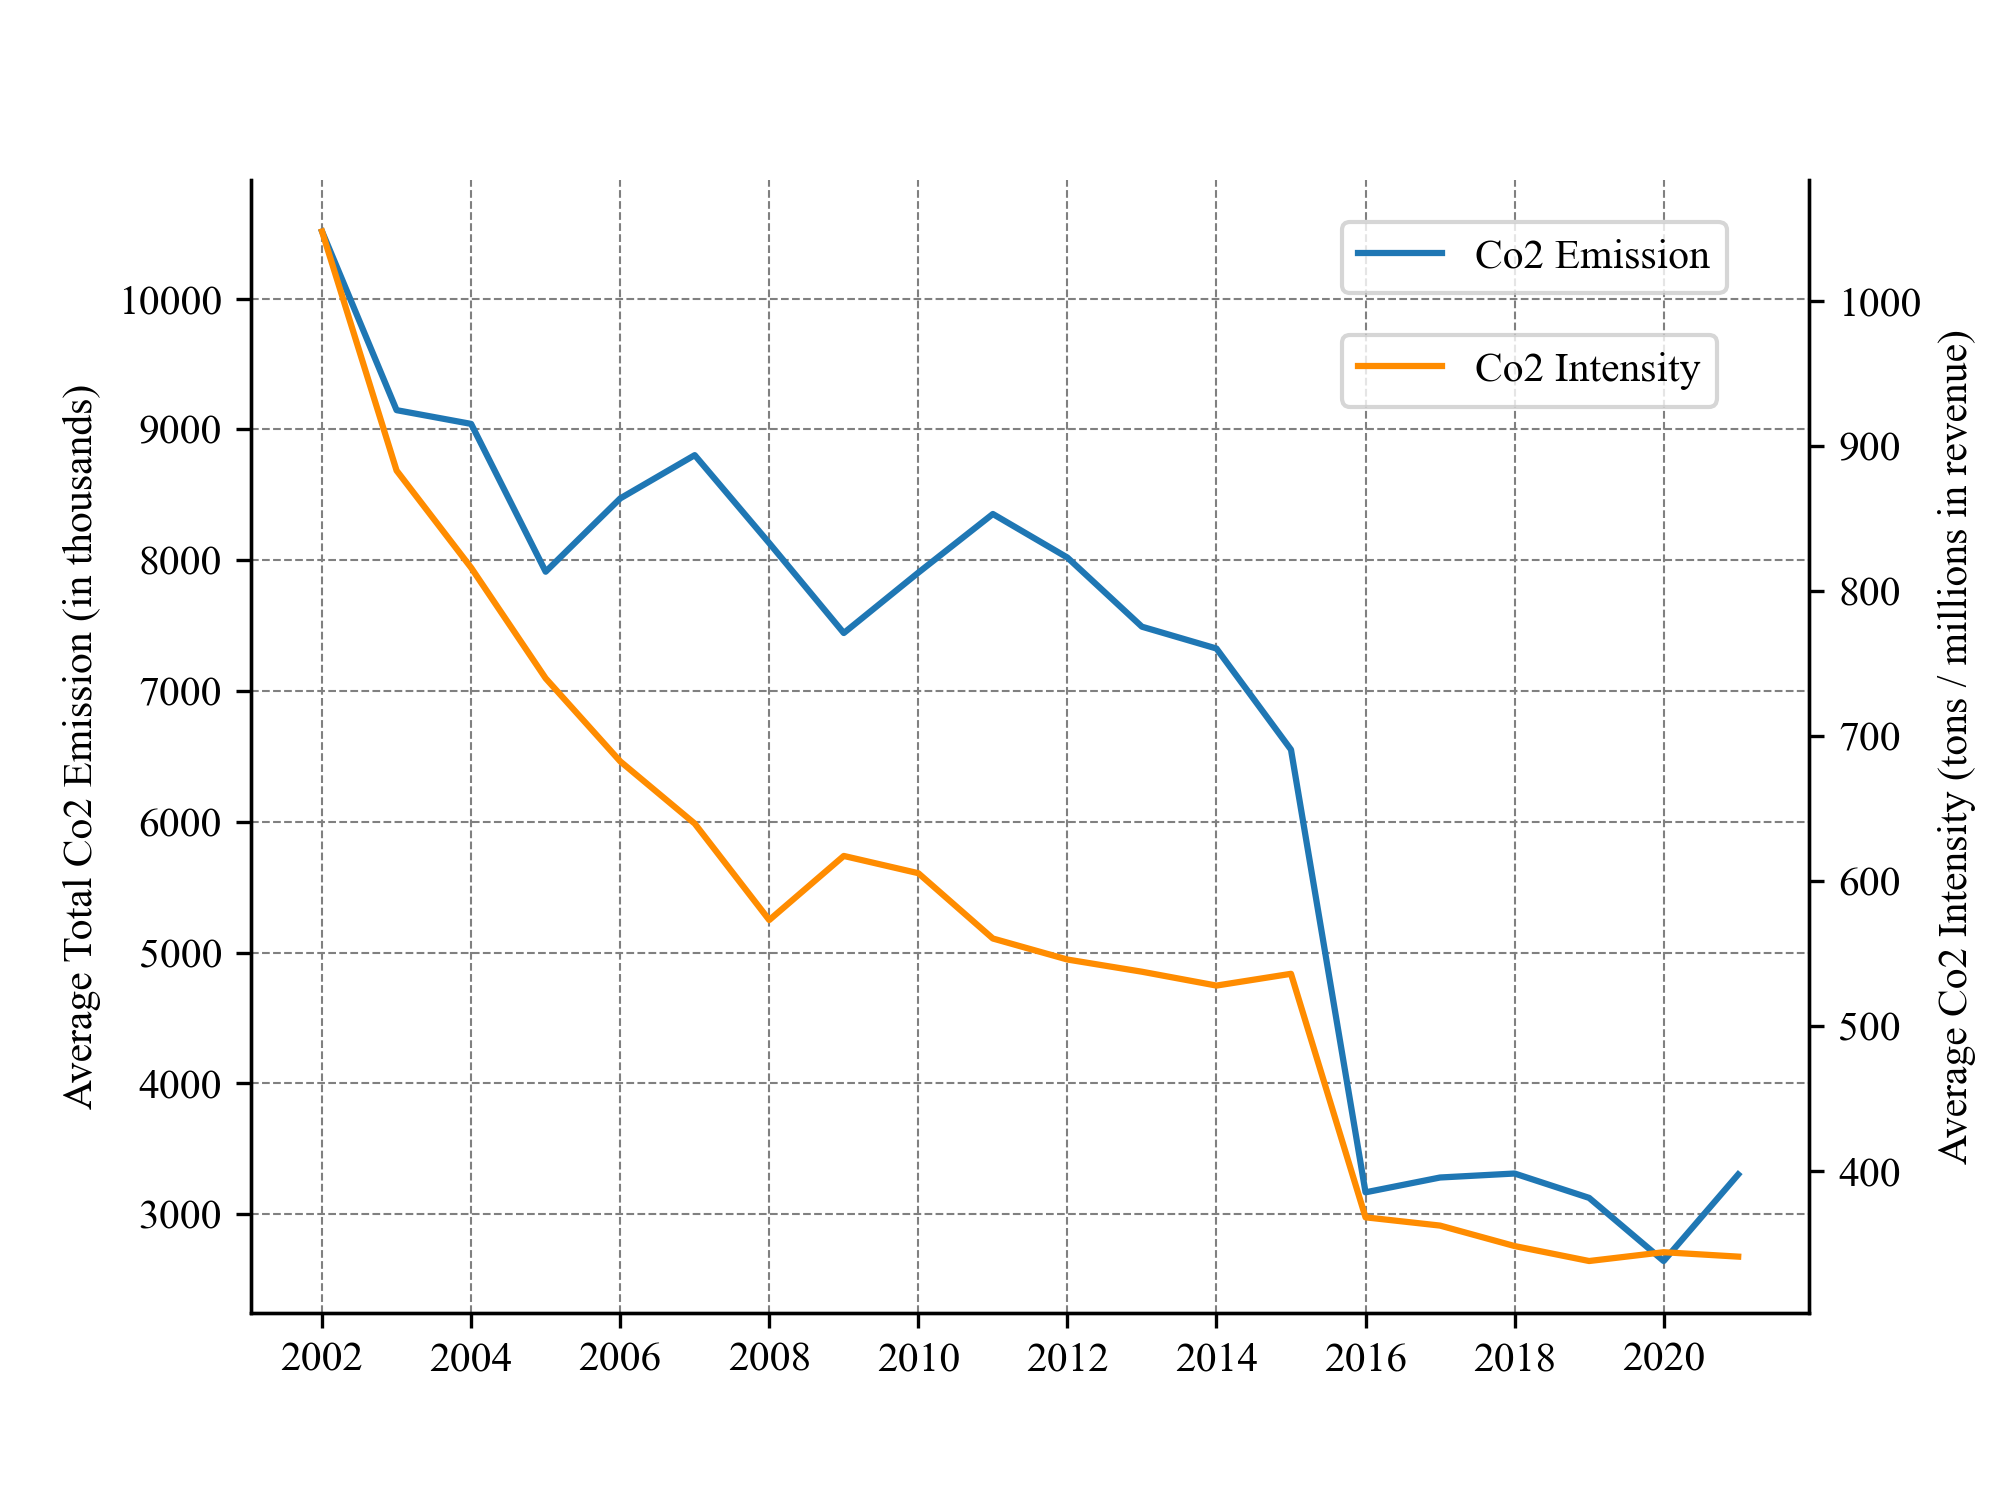
\includegraphics{graphics/co2_trend.png}
\label{fig: co2_intensity}
\caption*{\footnotesize{This graphic illustrates the historical trajectory of firms' total carbon emissions and intensity on average. Firms' total carbon emissions are measured in thousand tons, while intensity is quantified by tons of CO2 emitted per million US dollars of revenue. Both trajectories represent the mean value in each specific year.}}
\end{figure}

%%%%%%%%%%%%%%%%%%%%%%%%%%%%%%%%%%%%%%%%%%%%%%%%%%%
\subsection{Total Carbon Emissions in Different Industries}

Table \ref{tab: industries rank} provides a ranking of industries according to their average total carbon emissions over the period from 2002 to 2021. Notably, the industries with the most substantial average carbon emissions are Power and Renewable Electricity Productions, which exhibit an annual average of approximately 38.15 million tons. Electric Utilities and Oil, Gas, and Automobiles sectors secure the second and third positions, emitting around 37.46 million and 30.04 million tons of CO2 on average during the entire sampling period, respectively. These sectors are renowned for their notable environmental impacts due to the higher levels of carbon emissions they generate. On the contrary, industries with the least average carbon emissions encompass Industrial REITs, Health Care Technology, and Mortgage Real Estate Investment Trusts (REITs) sectors, showcasing relatively smaller environmental footprints based on their total carbon emissions. Taking into account the entire sampling period and a comprehensive range of industries, the average greenhouse gas emissions stand at 5.43 million tons. Strikingly, the most environmentally impactful sector, exemplified by Independent Power and Renewable Electricity Productions, demonstrates total CO2 emissions that are nearly 8 times higher than the average. In contrast, the most environmentally friendly industry, like Health Care Technology and Mortgage Real Estate Investment Trusts (REITs) sectors, emit only approximately 1/100th of the average emissions. This highlights a substantial diversity across industries concerning their total carbon emissions, underlining the significant heterogeneity in their environmental impacts.

%%%%%%%%%%%%%%%%%%%%%%%%%%%%%%%%%%%%%%%%%%%%%%%%%%
\begin{landscape}
\begin{table}[!ht]
\scriptsize
\centering
\caption{Industries Ranked by Average Total CO2 Emission}
\label{tab: industries rank}
\begin{tabular}{clcclc}
\toprule
 Rank &                                 GICS Industry Name &  Total CO2 Emission &  Rank &                               GICS Industry Name &  Total CO2 Emission \\
\midrule
1 & Power and Renewable Electricity Producers & 38.15 & 38 & Electronic Equipment, Instruments and Components & 1.23 \\
2 & Electric Utilities & 37.46 & 39 & Semiconductors and Semiconductor Equipment & 1.11 \\
3 & Automobiles & 30.04 & 40 & Specialty Retail & 1.09 \\
4 & Oil, Gas and Consumable Fuels & 28.28 & 41 & Textiles, Apparel and Luxury Goods & 1.08 \\
5 & Multi-Utilities & 21.05 & 42 & Construction and Engineering & 1.07 \\
6 & Passenger Airlines & 16.34 & 43 & Marine Transportation & 1.05 \\
7 & Construction Materials & 16.25 & 44 & Communications Equipment & 1.01 \\
8 & Industrial Conglomerates & 14.31 & 45 & Health Care Equipment and Supplies & 0.93 \\
9 & Metals and Mining & 13.48 & 46 & Trading Companies and Distributors & 0.86 \\
10 & Food Products & 12.75 & 47 & Leisure Products & 0.86 \\
11 & Financial Services & 10.05 & 48 & Specialized REITs & 0.82 \\
12 & Chemicals & 9.66 & 49 & IT Services & 0.78 \\
13 & Personal Care Products & 9.11 & 50 & Interactive Media and Services & 0.71 \\
14 & Consumer Staples Distribution and Retail & 7.62 & 51 & Distributors & 0.70 \\
15 & Household Products & 7.48 & 52 & Life Sciences Tools and Services & 0.63 \\
16 & Tobacco & 7.22 & 53 & Entertainment & 0.61 \\
17 & Aerospace and Defense & 6.28 & 54 & Media & 0.56 \\
18 & Air Freight and Logistics & 6.26 & 55 & Capital Markets & 0.45 \\
19 & Containers and Packaging & 6.25 & 56 & Insurance & 0.40 \\
20 & Beverages & 5.90 & 57 & Transportation Infrastructure & 0.36 \\
21 & Paper and Forest Products & 3.88 & 58 & Water Utilities & 0.31 \\
22 & Technology Hardware, Storage and Peripherals & 3.80 & 59 & Diversified Consumer Services & 0.29 \\
23 & Automobile Components & 3.72 & 60 & Banks & 0.26 \\
24 & Building Products & 2.90 & 61 & Professional Services & 0.23 \\
25 & Ground Transportation & 2.64 & 62 & Software & 0.21 \\
26 & Household Durables & 2.59 & 63 & Consumer Finance & 0.21 \\
27 & Machinery & 2.37 & 64 & Hotel and Resort REITs & 0.20 \\
28 & Diversified Telecommunication Services & 2.15 & 65 & Real Estate Management and Development & 0.18 \\
29 & Energy Equipment and Services & 2.07 & 66 & Health Care REITs & 0.17 \\
30 & Broadline Retail & 2.07 & 67 & Office REITs & 0.13 \\
31 & Wireless Telecommunication Services & 2.05 & 68 & Biotechnology & 0.11 \\
32 & Health Care Providers and Services & 2.00 & 69 & Retail REITs & 0.11 \\
33 & Pharmaceuticals & 1.91 & 70 & Diversified REITs & 0.11 \\
34 & Gas Utilities & 1.87 & 71 & Residential REITs & 0.09 \\
35 & Electrical Equipment & 1.40 & 72 & Industrial REITs & 0.06 \\
36 & Commercial Services and Supplies & 1.38 & 73 & Health Care Technology & 0.06 \\
37 & Hotels, Restaurants and Leisure & 1.31 & 74 & Mortgage Real Estate Investment Trusts (REITs) & 0.03 \\
\bottomrule
\end{tabular}
\begin{tablenotes}
\footnotesize
\item This table presents the ranking of different industries based on their average total CO2 emissions. The measurements for total CO2 emissions are provided in million tons. And the industry is categorized according to the GICS (Global Industry Classification Standard) industry classification.
\end{tablenotes}
\end{table}
\end{landscape}
\clearpage
%%%%%%%%%%%%%%%%%%%%%%%%%%%%%%%%%%%%%%%%%%%%%%%%%%%%%%%%%%%%%%%%
%%%%%%%%%%%%%%%%%%%%%%%%%%%%%%%%%%%%%%%%%%%%%%%%%%%%%%%%%%%%%%%%
\section{Result} \label{sec:result}

The main analysis of this paper tends to identify the relationship between firms' carbon emissions and their stock returns. To get the full picture of the story, we tend to do that in two steps. 
%%%%%%%%%%%%%%%%%%%%%%%%%%%%%%%%%%%%%%%%%%%%%%%%%%%
\subsection{Average Monthly Return on Firms' Carbon Footprint}

Our first practice delves into the unconditional relationship between firms' carbon footprint and their stock returns. Over the entire sample period, we adopt a cross-sectional approach, sorting carbon emissions into 100 percentiles. Within each percentile, we compute the average monthly stock returns to gain an overarching understanding of the link between firms' carbon emissions and their stock performance. Figure \ref{fig: co2_percentile} visually presents these findings. Panel A focuses on the average stock returns concerning firms' total carbon emissions, while panels B, C, and D examine emissions within different emission scopes. Across all four panels, a distinguished downward trend emerges, indicating that firms with higher carbon emissions tend to exhibit lower stock returns on average. Additionally, we observe peaks in average stock returns occurring when firms' carbon emissions fall around the 1st percentile for all scopes. Another set of peaks in average returns is notable for different emissions categories, such as total carbon emissions around the 58th percentile, scope 1 emissions near the 65th percentile, scope 2 emissions at approximately the 79th percentile, and scope 3 emissions around the 55st percentile. These clusters of companies may share common characteristics, possibly belonging to the same industry, with similarities in terms of size, profitability, and growth. It's important to note that in this analysis, we specifically sort firms based on their carbon emissions only, without considering other stock return-related factors. Nevertheless, these initial findings provide valuable insights into the preliminary relationship between firms' carbon emissions and their realized stock returns.

\begin{figure}[!ht]
\centering
\caption{\textbf{Average Stock Returns Based on Carbon Emissions}}
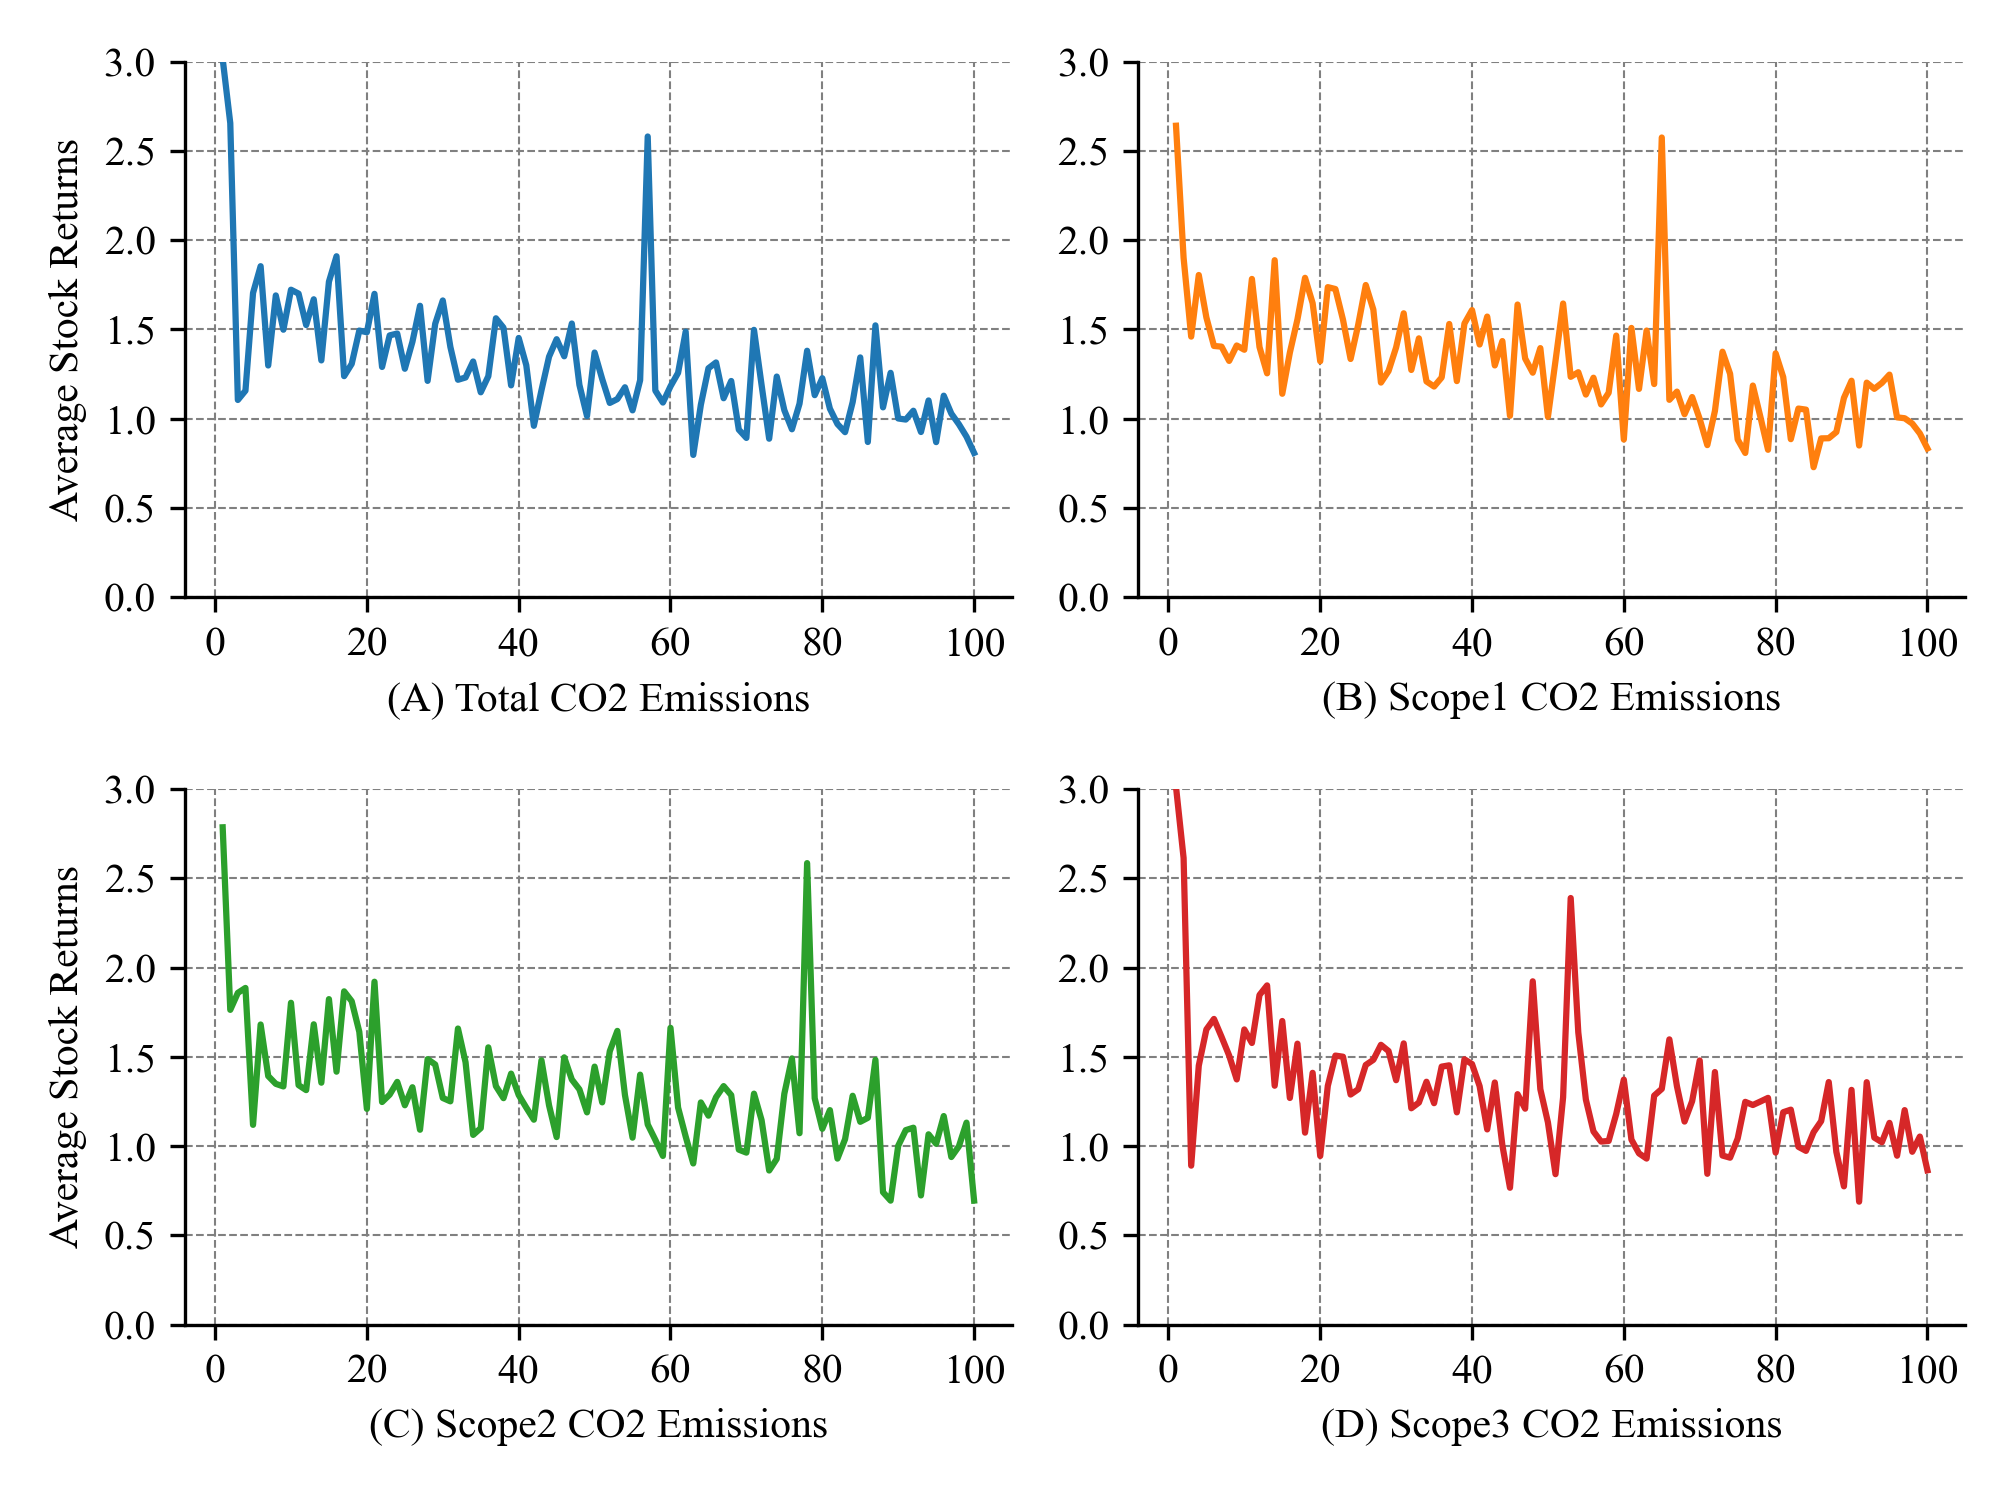
\includegraphics{graphics/co2_percentile.png}
\label{fig: co2_percentile}
\caption*{\footnotesize{This presents the average monthly stock returns in relation to different percentiles of carbon emissions. Panel A depicts the average stock return in relation to firms' total carbon emissions, while Panel B illustrates the average stock return concerning firms' scope 1 carbon emissions. Panel C showcases the average stock return with respect to firms' scope 2 carbon emissions, and Panel D presents the average stock return in connection with firms' scope 3 carbon emissions.}}
\end{figure}

Following the same analytical approach, we explore whether a similar pattern emerges with another crucial indicator in corporate finance literature pertaining to firms' carbon footprint. Figure \ref{fig: intensity_percentile} illustrates the average monthly stock returns across different percentiles of firms' carbon intensity. In contrast to the previous analysis of carbon emissions, we do not discern a clear and consistent trend in firms' average monthly stock returns across all four panels, where each representing different scopes of firms' carbon intensity. The absence of a discernible trend suggests that the relationship between firms' carbon intensity and their stock returns may not exhibit the same patterns as strongly as observed with carbon emissions. 

\begin{figure}[!ht]
\centering
\caption{\textbf{Average Stock Returns Based on Carbon Intensity}}
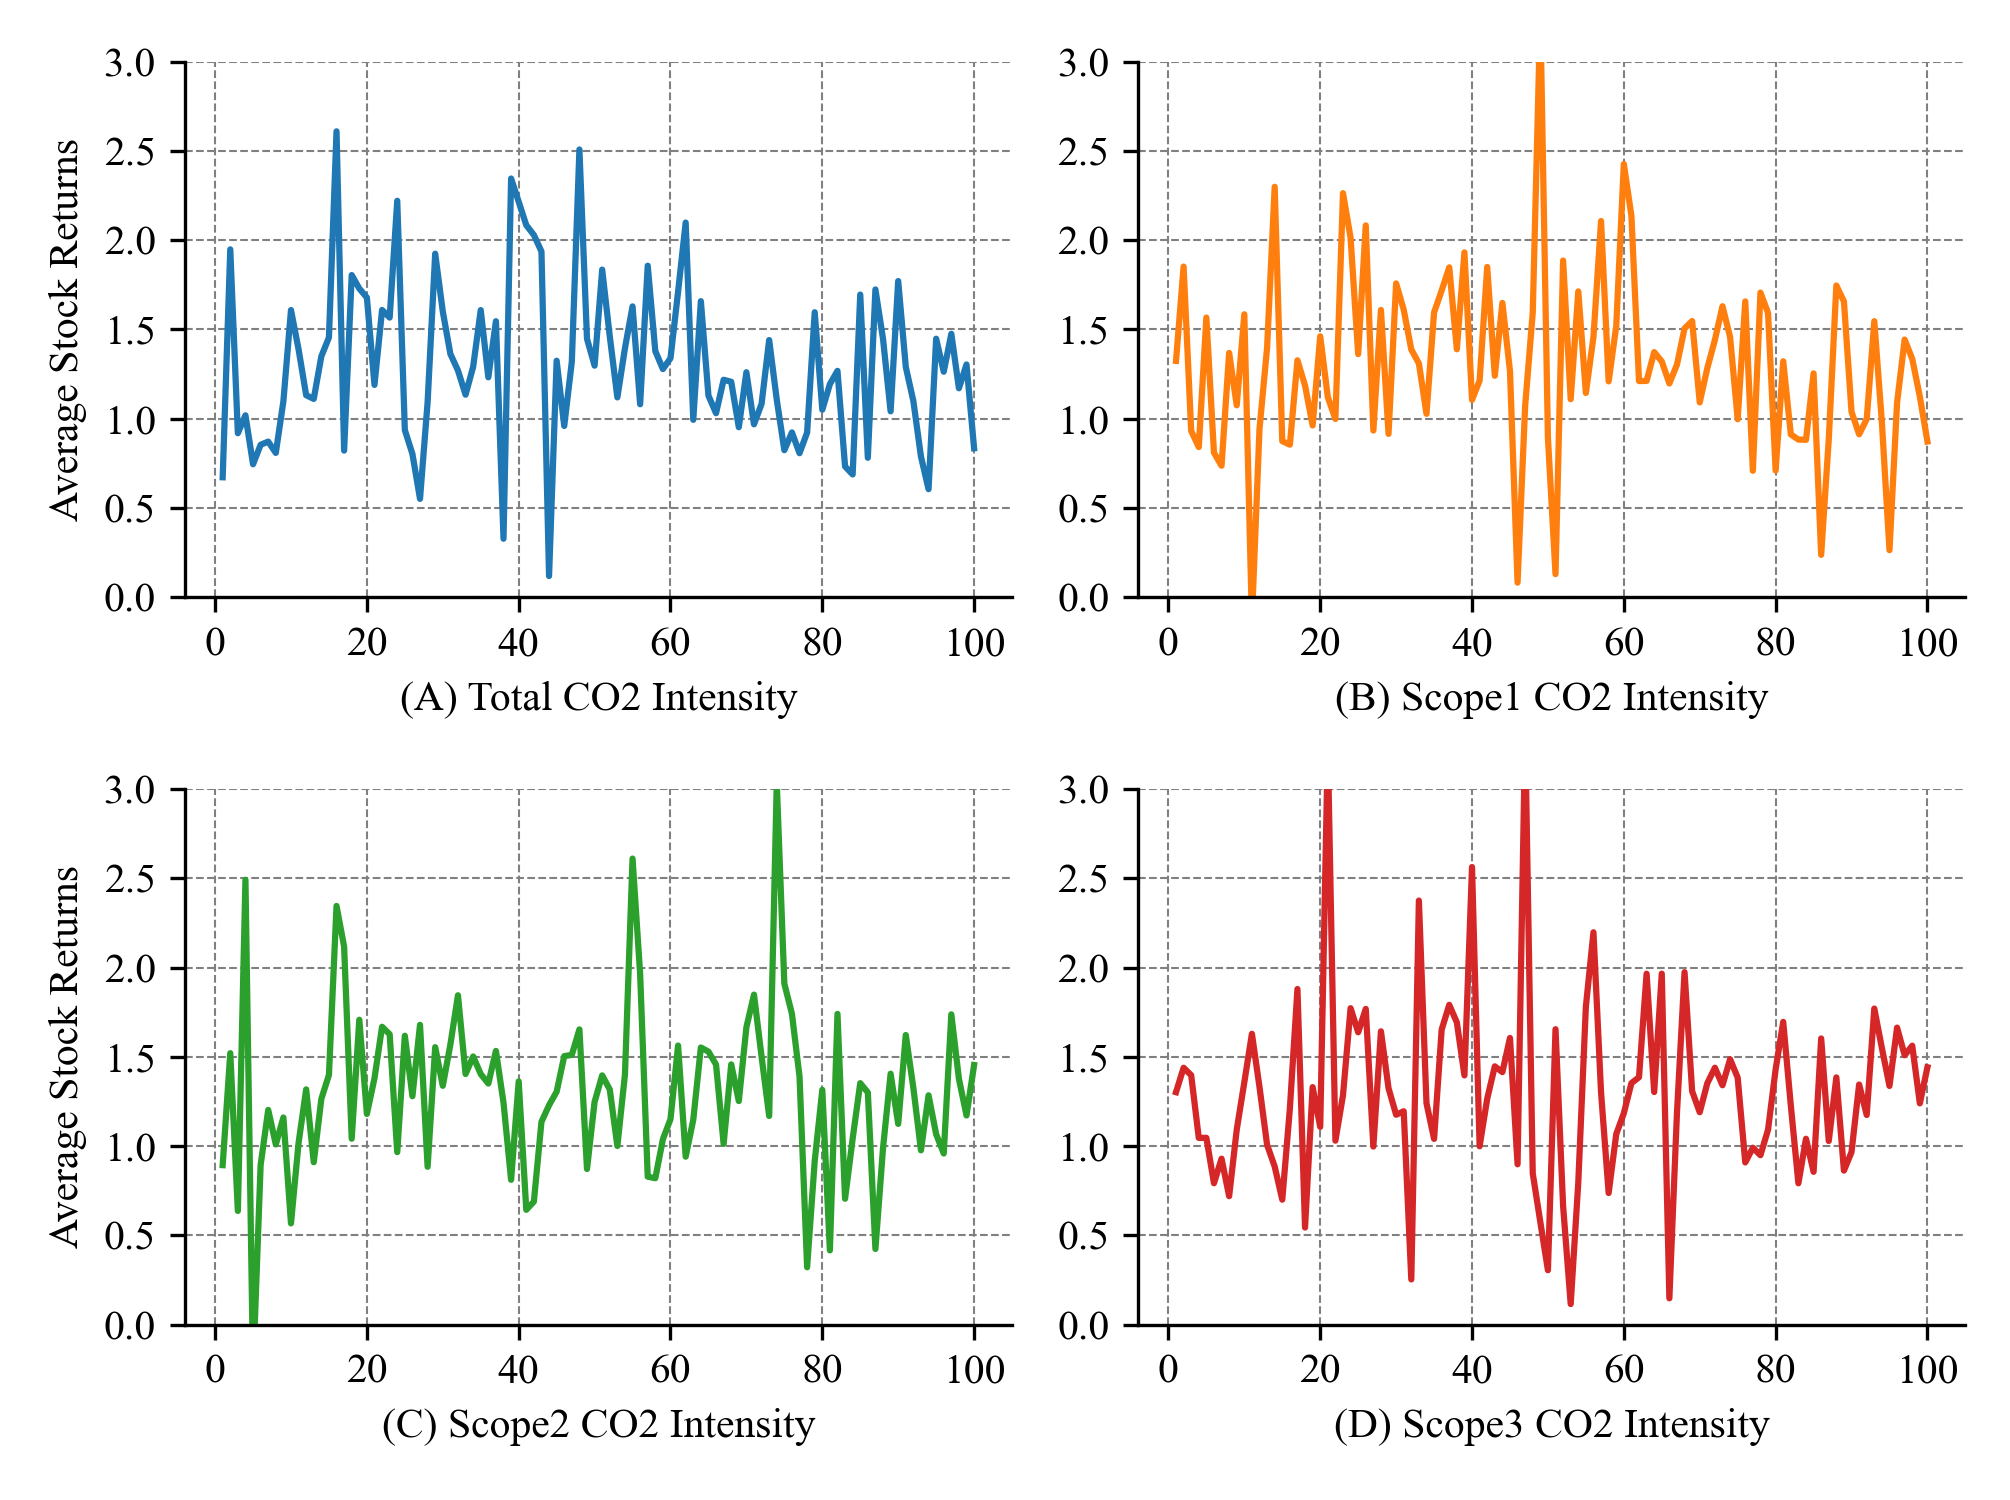
\includegraphics{graphics/int_percentile.png}
\label{fig: intensity_percentile}
\caption*{\footnotesize{This presents the average monthly stock returns in relation to different percentiles of carbon intensity. Panel A depicts the average stock return in relation to firms' total carbon intensity, while Panel B illustrates the average stock return concerning firms' scope 1 carbon intensity. Panel C showcases the average stock return with respect to firms' scope 2 carbon intensity, and Panel D presents the average stock return in connection with firms' scope 3 carbon intensity.}}
\end{figure}

Similar patterns are not observered when plotting other key firm characteristics alongside stock returns. Some may raise concerns that that the cross-sectional relationship between firms' stock returns and carbon emissions could be influenced by confounding factors such as firm size, leverage, profitability, and growth, as illustrated in Table \ref{tab: corr} the strong correlation between firms' carbon emissions and some characteristic variables. Notably, the high and statistically significant positive correlation between firms' carbon emissions and size. To address these concerns, we present the average monthly stock returns in relation to various firms' characteristics in Figure \ref{fig: others_persentile}. In panel (A), we observe a positive association between firm size and stock returns within the first 20 percentiles; however, beyond this range, the relationship becomes less apparent. It is important to remember that firm size has a high correlation with carbon emissions. The most similar pattern emerges from the plot between leverage and stock return, however the correlation between leverage and carbon emission only is 0.09. While other patterns emerge in stock returns concerning variables like RoE and revenue growth, it's essential to note that these variables exhibit weak correlations with firms' carbon emissions.
\begin{figure}[!ht]
\centering
\caption{\textbf{Average Stock Returns Based on Other Indicators}}
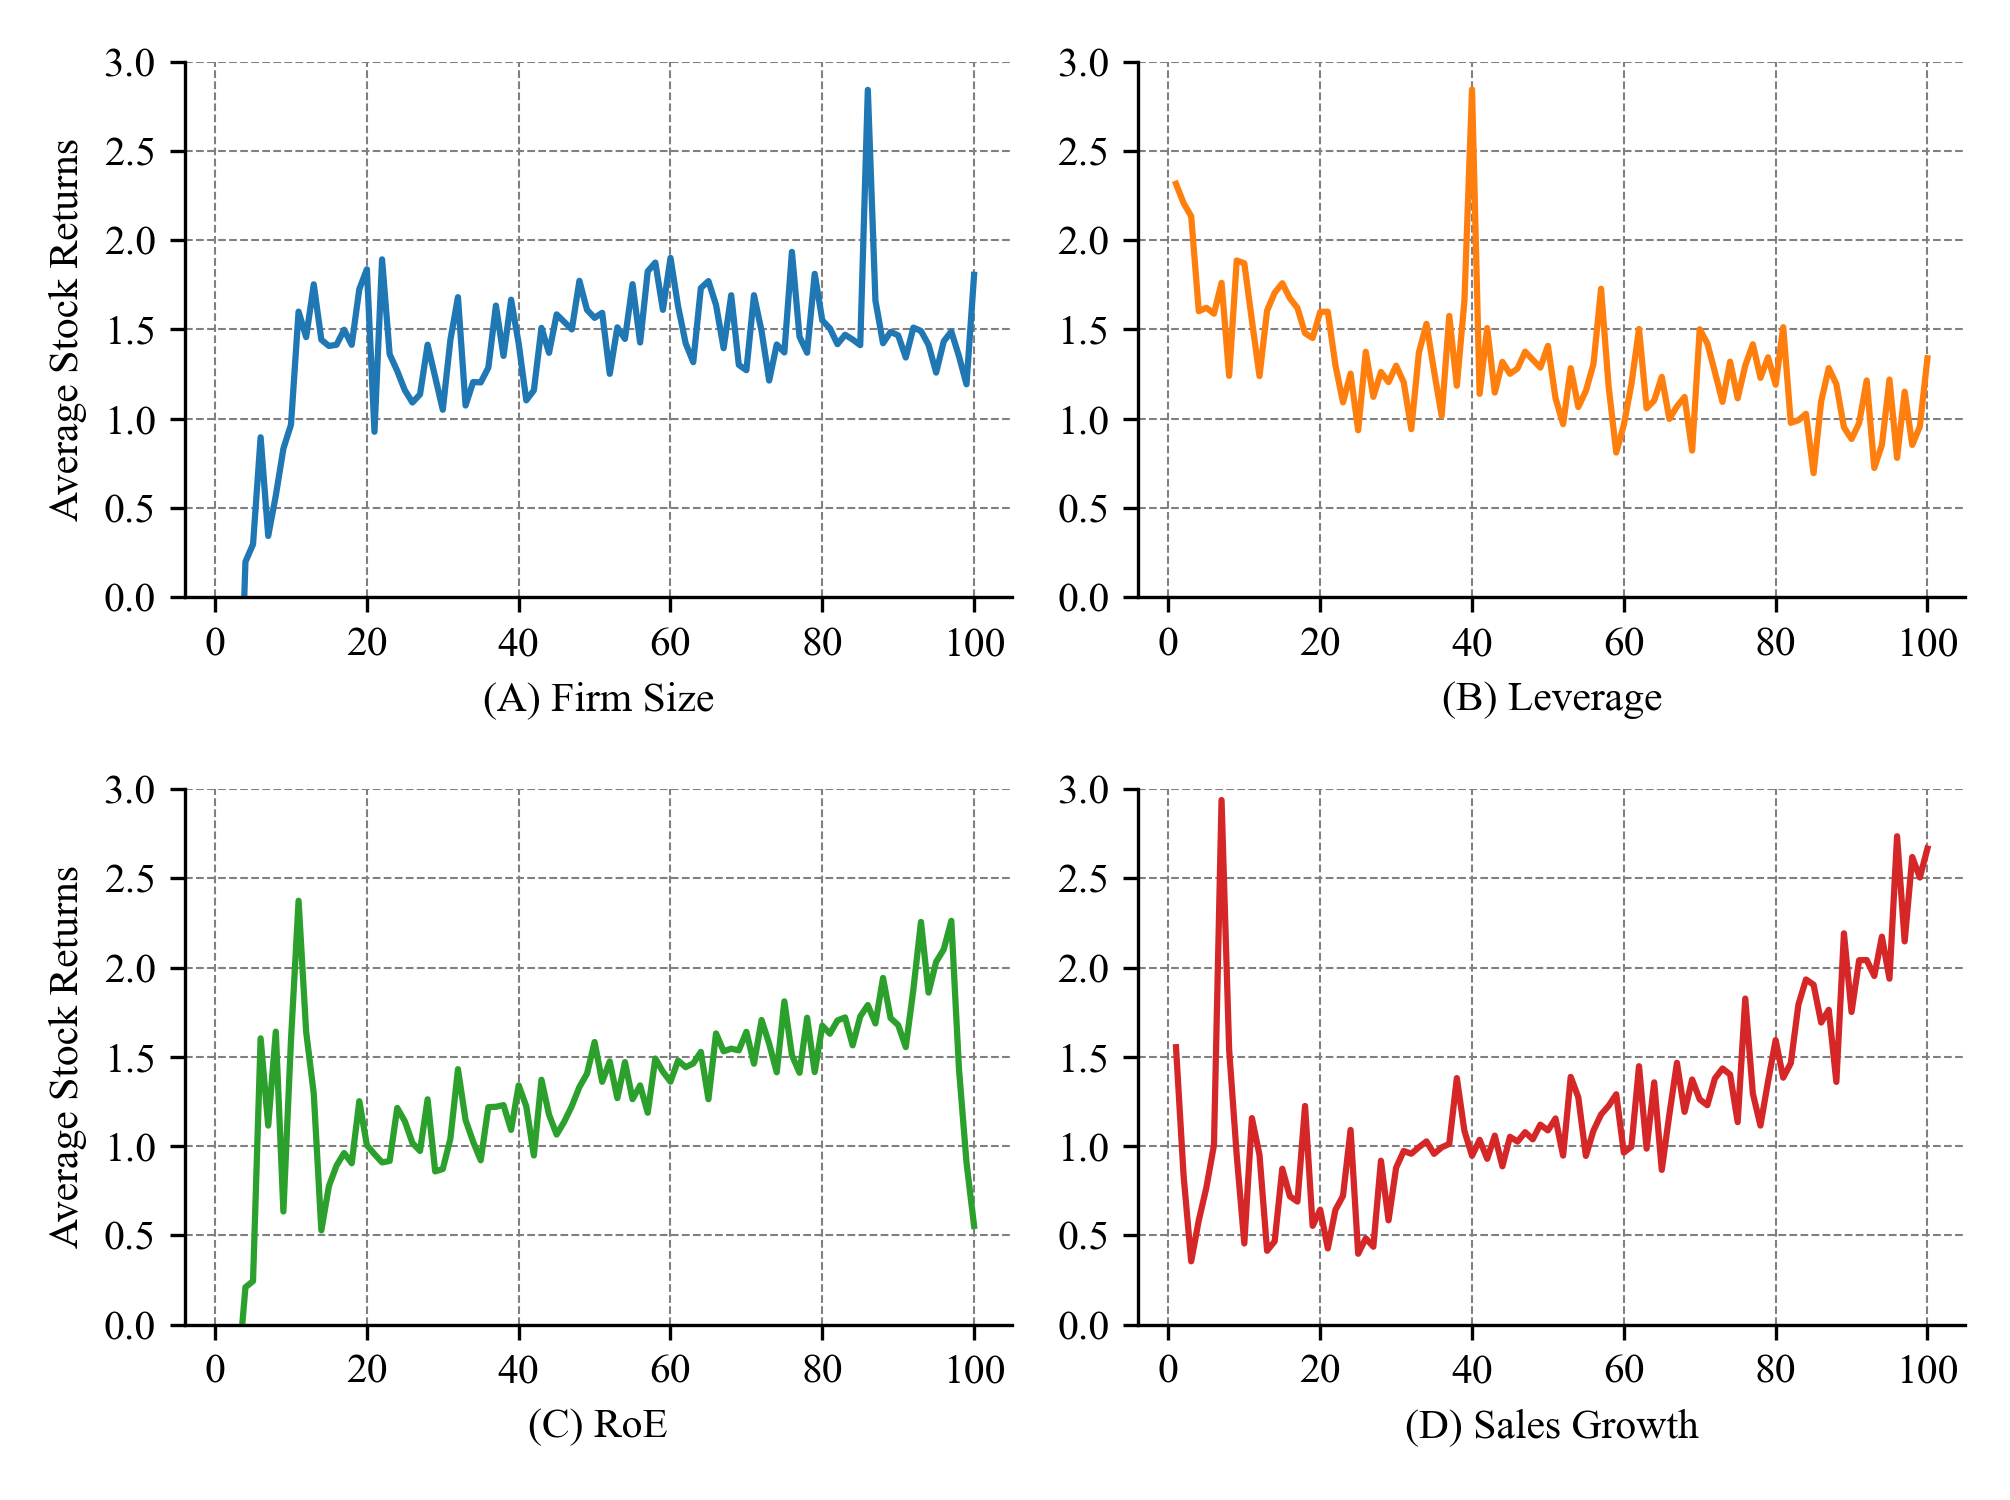
\includegraphics{graphics/other_percentile.png}
\label{fig: others_persentile}
\caption*{\footnotesize{This presents the average monthly stock returns in relation to different percentiles of various firms' characteristic indicators. Panel A depicts the average stock return in relation to firms' market capitalization, while Panel B illustrates the average stock return concerning firms' leverage. Panel C showcases the average stock return with respect to firms' profitability ROE, and Panel D presents the average stock return in connection with firms' growth in revenue.}}
\end{figure}


%%%%%%%%%%%%%%%%%%%%%%%%%%%%%%%%%%%%%%%%%%%%%%%%%%%
\subsection{Realized Cumulative Return for Green and Brown Portfolios}

The green portfolio outperform its brown counterpart over the entire sample period, with firm total carbon emissions determining their categorization. Following the methodology presented in Equation \ref{eqn: measure greenness}, we sort stocks into quintiles monthly based on their industry-specific carbon emissions. Generally, firms with higher emissions, categorized as brown, are those exceeding the 80th percentile in carbon emissions due to their significant environmental impact. Conversely, firms below the 20th percentile are assigned to the green portfolio. Those between the 40th and 60th percentiles are placed in the neutral portfolio. Firms falling between the 20th and 40th percentiles, as well as those between the 60th and 80th, are excluded for a clearer comparison. The green portfolio demonstrates superior cumulative realized returns, as depicted in Figures \ref{fig: cum_ret_1} for the period from 2002 to 2021. Each portfolio is value-weighted based on the market capitalization of the included firms to ensure fairness and accuracy\footnote{In the portfolio analysis we use the data without manipulation. Since the outliers are often observed in samll-cap stocks and portfolio is constructed by value weighted, so the influence of these outliers will be minimized. And the the un-manipulated data help us aviod the critisim of data manipulation.}. Notably, portfolio reallocation is an annual process due to the yearly update of firms' carbon emission data, allowing us to disregard transaction fees in this analysis. At the end of the sample period the brown portfolio realized less than 300\% cumulative returns, while the green portfolio realized cumulative returns more than 600\% twice higher its brown counterpart.

\begin{figure}[!ht]
\centering
\caption{\textbf{Cumulative Portfolio Return by Carbon Emissions}}
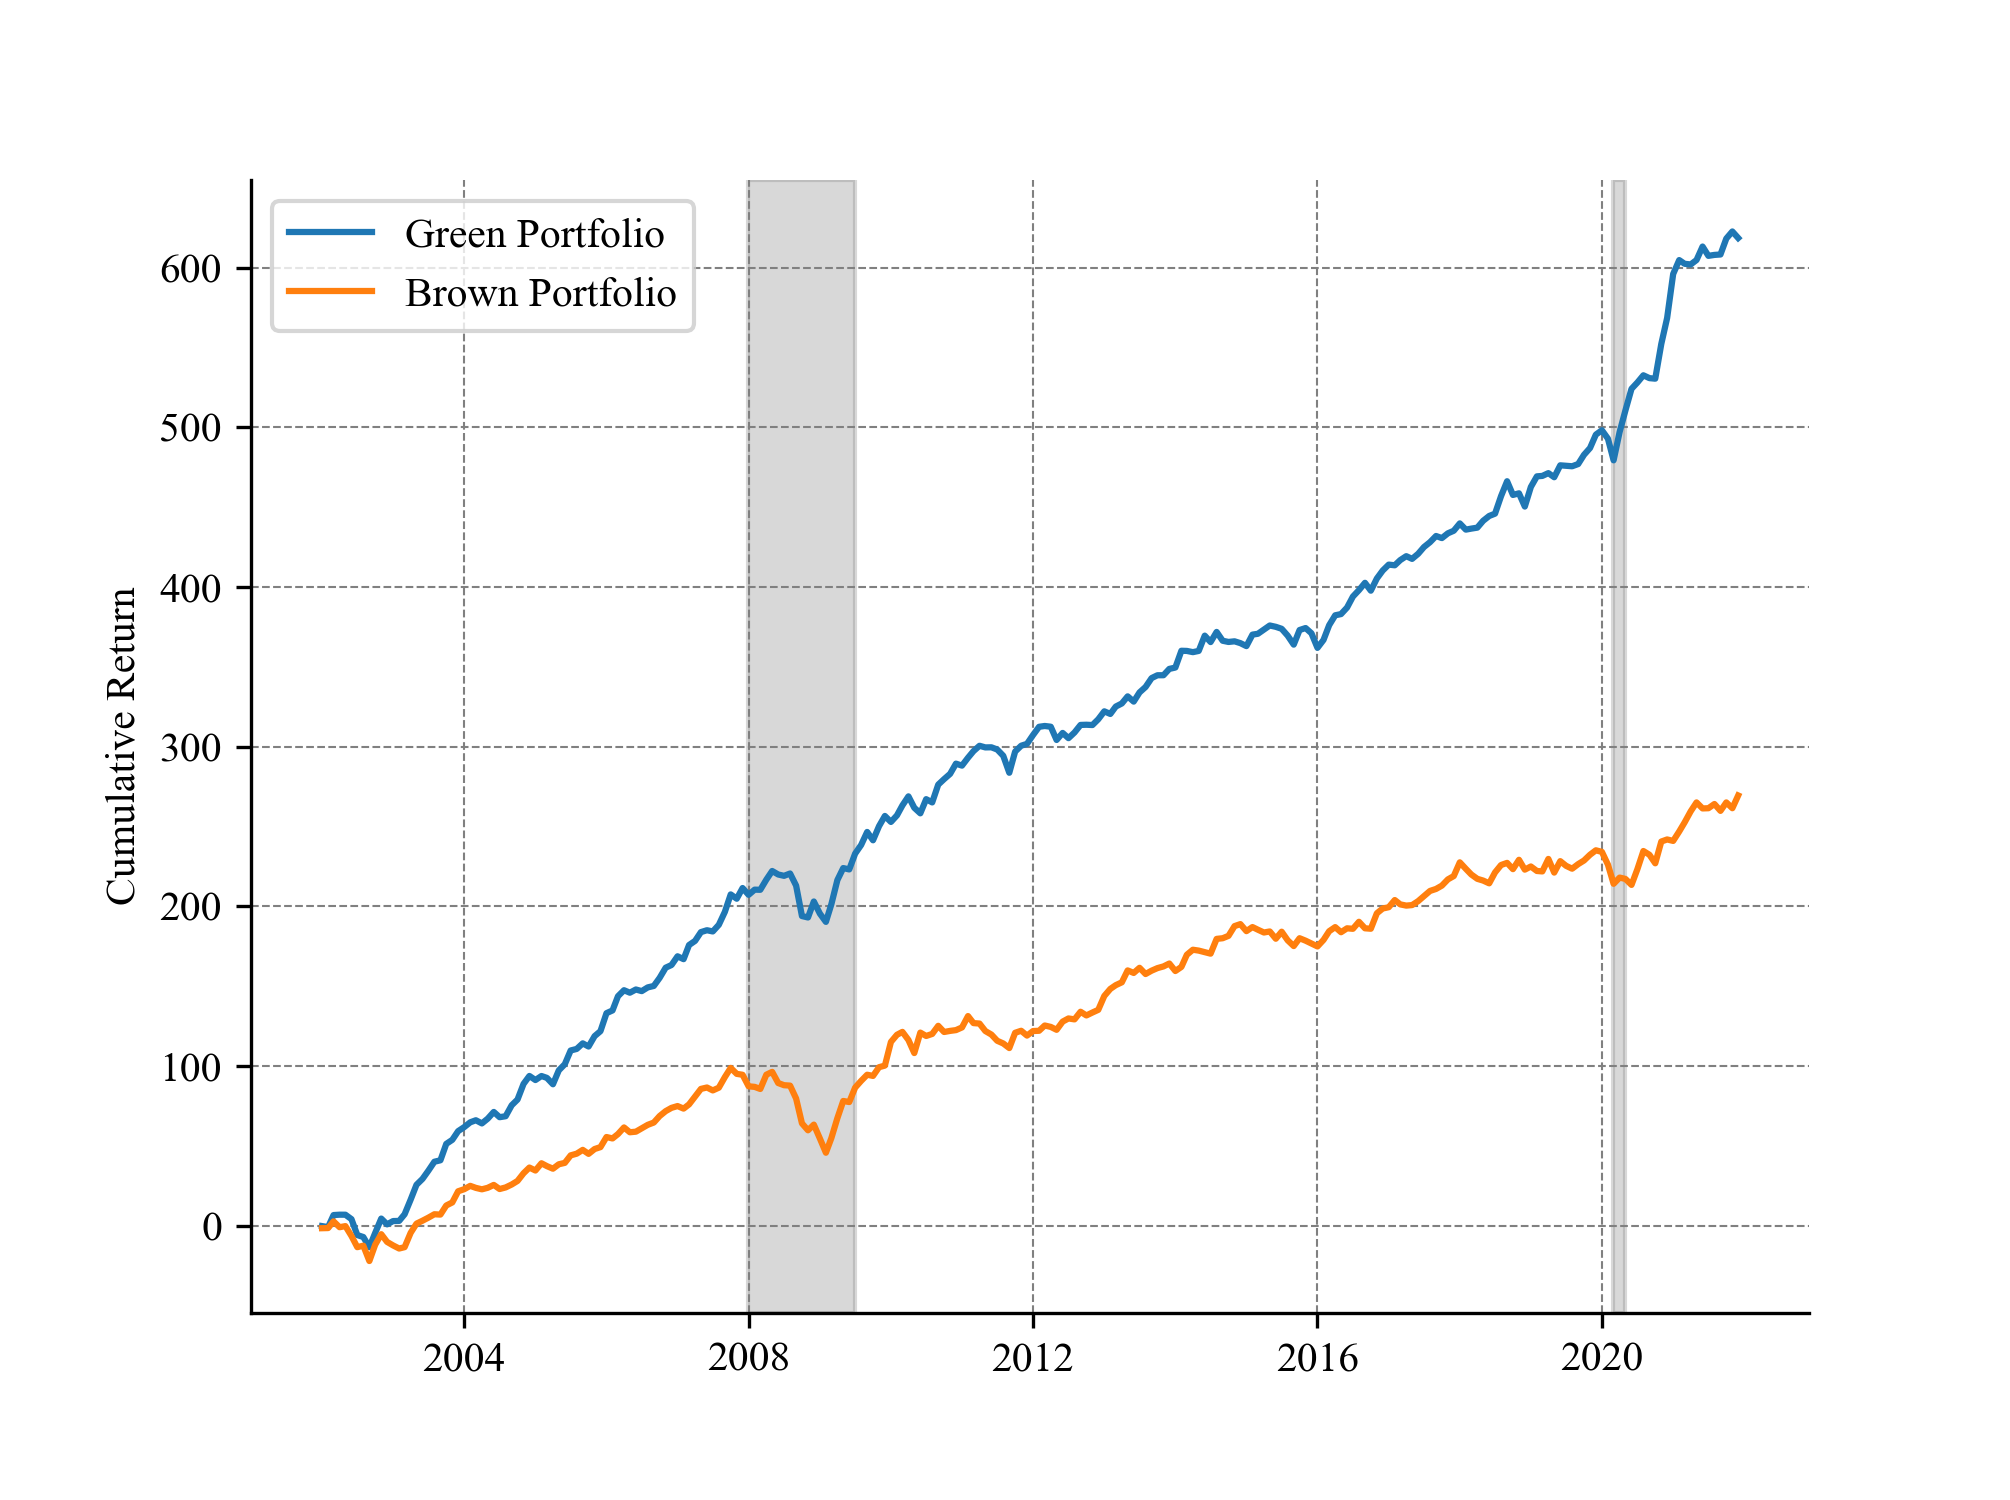
\includegraphics{graphics/green_brown_co2.png}
\label{fig: cum_ret_1}
\caption*{\footnotesize{This graphic illustrates the historical trajectory of firms' total carbon emissions and intensity. Firms' total CO2 emissions are measured in thousand tons, while intensity is quantified by tons of carbon emitted per million US dollars of revenue.}}
\end{figure}

The green portfolio, categorized based on firms' carbon intensity, shows only slight outperformance compared to its brown counterpart, and this outperform is observed only after 2011. Following the same methodology, we group stocks into green and brown groups based on their carbon intensity. The cumulative returns of these portfolios are presented in Figure \ref{fig: cum_ret_2}. Throughout the entire sample period, the green portfolio achieves a cumulative return of approximately 400\%, and its brown counterpart realizes a cumulative return around 300\%. Notably, the green portfolio's outperformance is only evident post-2011; prior to this, both portfolios exhibited similar cumulative return trajectories.

\begin{figure}[!ht]
\centering
\caption{\textbf{Cumulative Portfolio Returns by Intensity}}
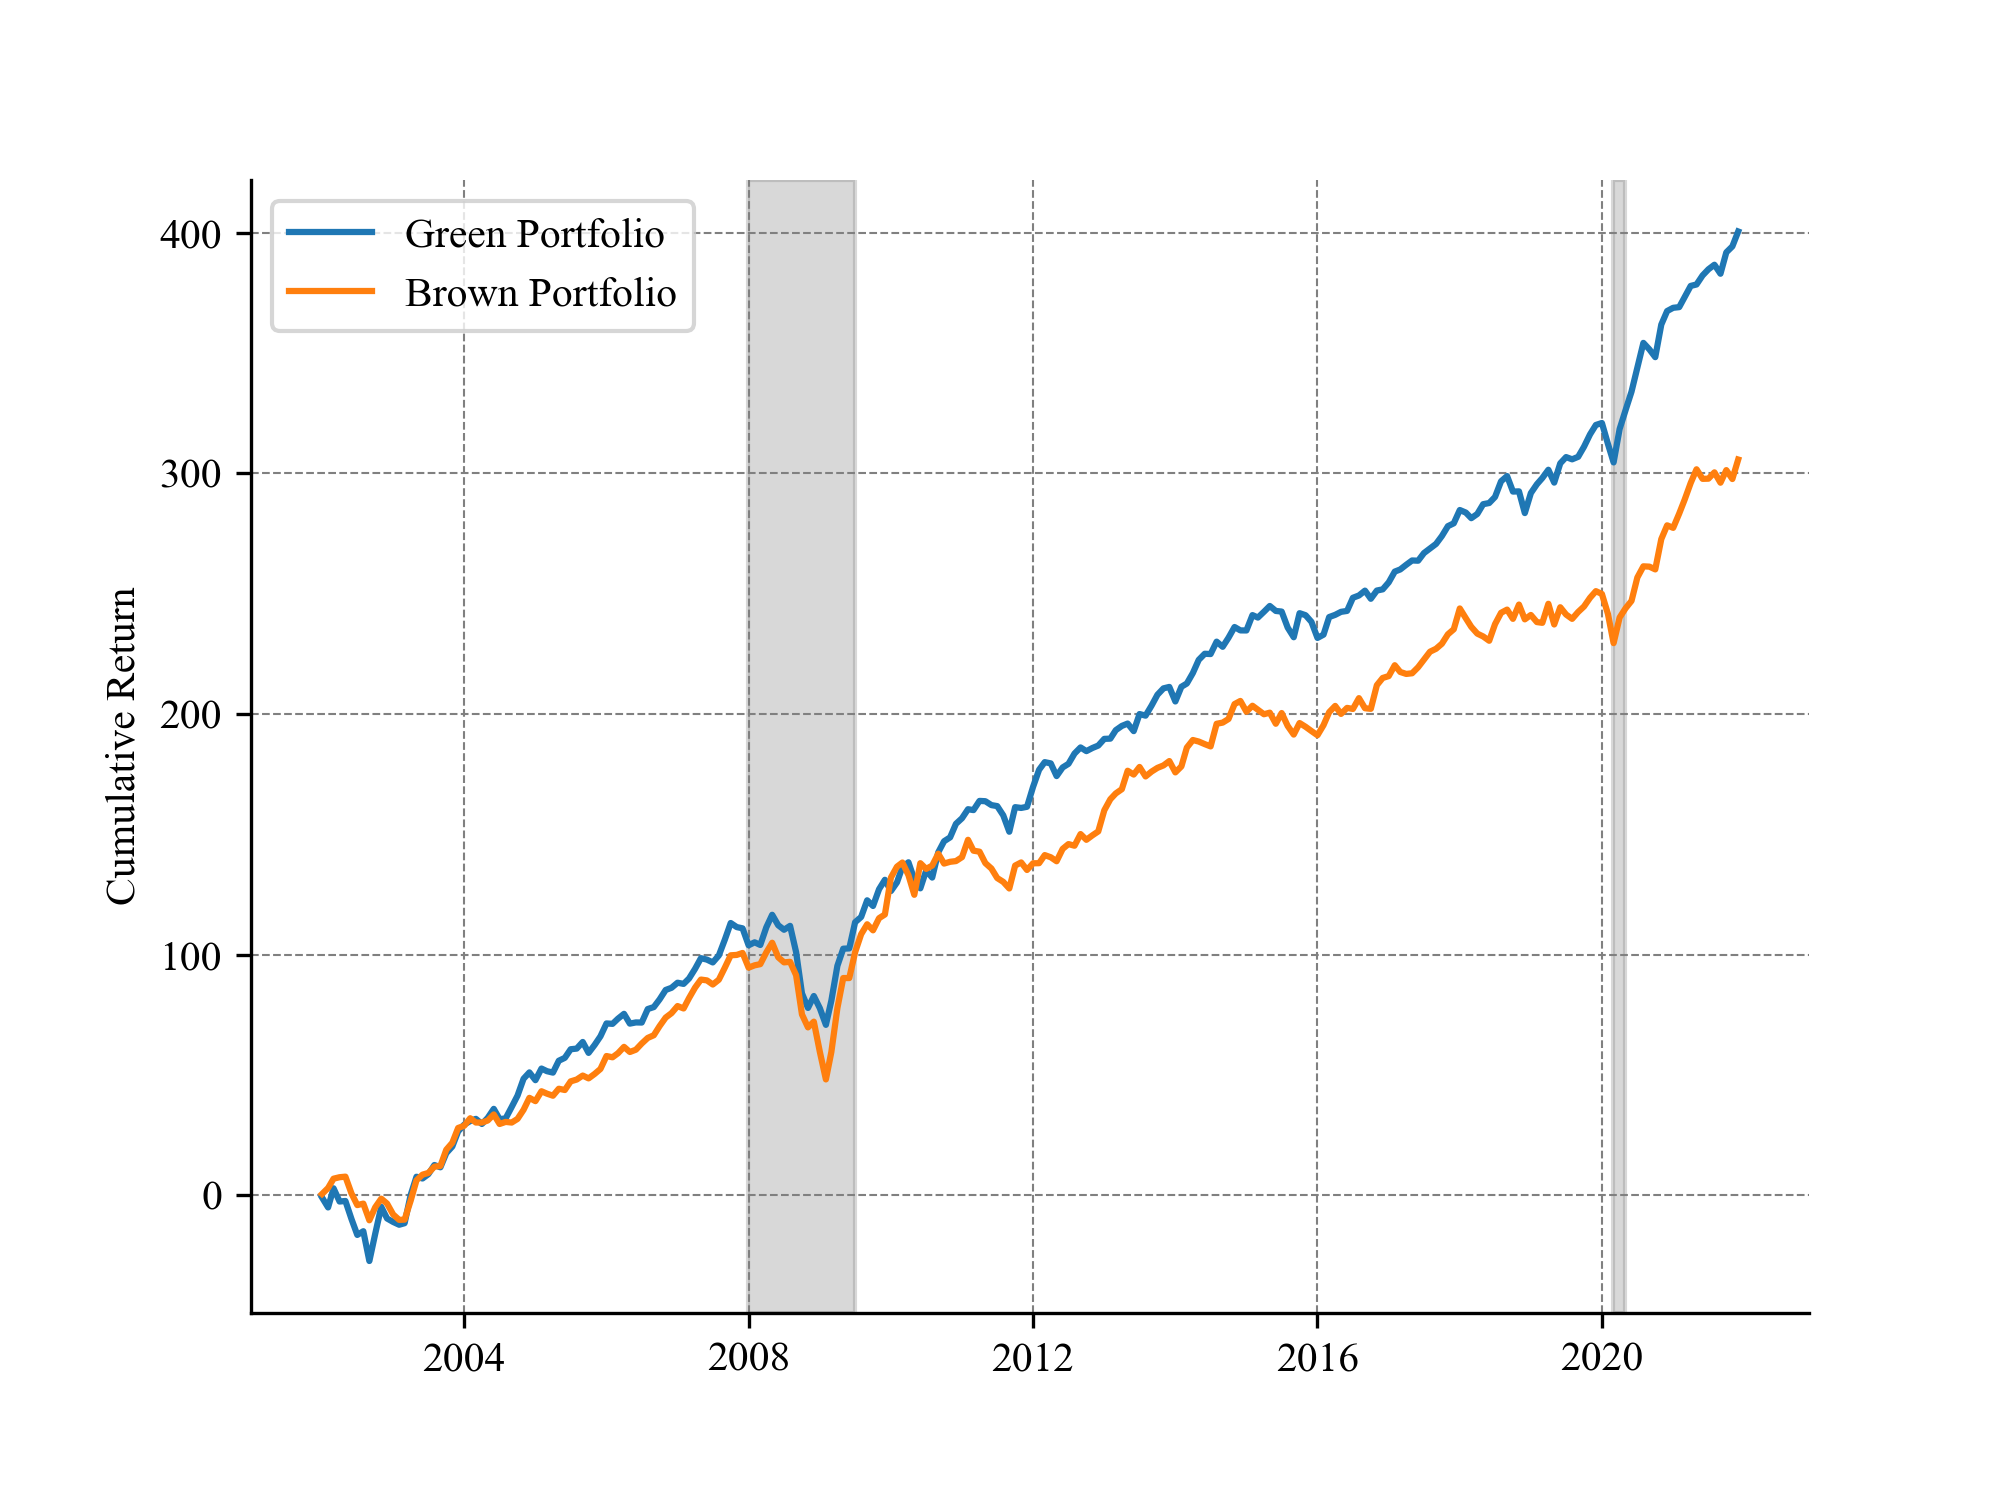
\includegraphics{graphics/green_brown_int.png}
\label{fig: cum_ret_2}
\caption*{\footnotesize{This graphic illustrates the historical trajectory of firms' total carbon emissions and intensity. Firms' total CO2 emissions are measured in thousand tons, while intensity is quantified by tons of carbon emitted per million US dollars of revenue.}}
\end{figure}

%%%%%%%%%%%%%%%%%%%%%%%%%%%%%%%%%%%%%%%%%%%%%%%%%%%
\subsection{The Green-Brown Premium}


Tak inspiration from \cite{pastor2022dissecting}, we introduce the concept of the GMB (Green Minus Brown) premium, quantified as the monthly difference between the return of Green and Brown portfolios. This discrepancy is elaborated in Table \ref{tab: green-brown}, wherein the first column showcases the GMB premium originating from firms' overall carbon emissions. Notably, the intercept is 44.3 basis points (bp), accompanied by a corresponding standard error of 25.3 bp. This suggests that, on average, the Green portfolio outperforms the Brown counterpart by approximately 44.3 bp per month. Importantly, this difference exhibits statistical significance at the 10\% level. In contrast, the fourth column of Table \ref{tab: green-brown} elucidates the GMB premium derived from firms' CO2 intensity. Notably, in this case, the Green portfolio demonstrated no noteworthy outperformance against the Brown portfolio. The average stands at a mere 0.4 basis points per month, accompanied by a standard error of 26.3 bp, which is not significant either economically or statistically.

In columns 2 and 3 of Table \ref{tab: green-brown}, we regress the GMB portfolio's return on the Fama-French 3 and 5 factors model, as discussed by \cite{fama2015five} and \cite{fama1993common}, the results show mixed evidence. With the Fama-French 5 factors model, we still get a significant positive intercept. This finding suggests that there is still an unexplained risk premium by the classical factor models. But with the Fama-French 3 factors model even if the intercept is still positive it becomes statistically insignificant.\footnote{In the paper by \cite{pastor2022dissecting}, they use E score from ESG rating to formulate GMB portfolio and find better empirical results, where all the intercepts are statistically and economically significant.} When we formulate the GMB portfolio by firms' carbon intensity, all the intercepts from different regression models become both economically and statistically insignificant as shown in columns 4-6 in Table \ref{tab: green-brown}. The pivotal distinction between shaping the portfolio using total carbon emissions versus intensity emerges as a noteworthy finding. Empirical evidence underscores the superiority of total carbon emissions as a more robust indicator for quantifying firms' greenness. This empirical inclination emerges despite the seemingly logical construct of carbon intensity. As it stands, the data does not substantiate carbon intensity's position as a superior greenness indicator.
%%%%%%%%%%%%%%%%%%%%%%%%%%%%%%%%%%%%%%%%%%%%%%%%%%%

\begin{table}[!ht]
\centering
\footnotesize
\caption{Green - Brown Portfolios Regress on Factors}
\label{tab: green-brown}
{
\def\sym#1{\ifmmode^{#1}\else\(^{#1}\)\fi}
\begin{tabular}{@{\extracolsep{2pt}}l*{8}{c}@{}}
\toprule
& \multicolumn{4}{c}{CO2 Emission} & \multicolumn{4}{c}{Intensity} \\
\cline{2-5}
\cline{6-9}
               & Model 1  & Model 2   & Model 3   & Model 4   & Model 5 & Model 6   & Model7    & Model8     \\
\hline
Intercept      & 1.454*** & 1.169***  & 1.181***  & 1.073***  & 0.395*  & 0.124     & 0.080     & 1.073***   \\
               & (0.319)  & (0.268)   & (0.280)   & (0.298)   & (0.234) & (0.209)   & (0.218)   & (0.298)    \\
Mkt\_RF        &          & 0.072     & 0.070     & 0.120     &         & 0.251***  & 0.266***  & 0.120      \\
               &          & (0.065)   & (0.069)   & (0.073)   &         & (0.051)   & (0.054)   & (0.073)    \\
SMB            &          & 1.092***  & 1.078***  & 1.039***  &         & 0.199**   & 0.200**   & 1.039***   \\
               &          & (0.113)   & (0.119)   & (0.119)   &         & (0.088)   & (0.092)   & (0.119)    \\
HML            &          & -0.543*** & -0.554*** & -0.470*** &         & -0.575*** & -0.625*** & -0.470***  \\
               &          & (0.100)   & (0.114)   & (0.119)   &         & (0.078)   & (0.089)   & (0.119)    \\
RMW            &          &           & -0.045    & -0.112    &         &           & 0.030     & -0.112     \\
               &          &           & (0.138)   & (0.140)   &         &           & (0.107)   & (0.140)    \\
CMA            &          &           & 0.062     & 0.071     &         &           & 0.173     & 0.071      \\
               &          &           & (0.182)   & (0.181)   &         &           & (0.142)   & (0.181)    \\
MOM            &          &           &           & 0.178**   &         &           &           & 0.178**    \\
               &          &           &           & (0.076)   &         &           &           & (0.076)    \\
LIQ            &          &           &           & -2.381    &         &           &           & -2.381     \\
               &          &           &           & (4.143)   &         &           &           & (4.143)    \\

\hline
Obs & 240 & 240 & 240 & 240 & 240 & 240 & 240 & 240 \\
R-squared      & 0.000    & 0.327     & 0.327     & 0.343     & -0.000  & 0.243     & 0.248     & 0.343      \\
\bottomrule
\multicolumn{7}{l}{\footnotesize * p\sym{<}.1, ** p\sym{<}.05, *** p\sym{<}.01}
\end{tabular}
}
\begin{tablenotes}
    \item This table presents the regression results of the Green minus Brown portfolio on different factor models. In the left panel, the portfolio is formulated based on firms' total carbon emissions, and in the right panel, the portfolio is based on firms' carbon intensity. Columns 1 and 4 only show regression results with intercept, columns 2 and 5 show regression results with Fama-French 3 factors model, and columns 3 and 6 show regression results with Fama-French 5 factors model.
\end{tablenotes}
\end{table}

%%%%%%%%%%%%%%%%%%%%%%%%%%%%%%%%%%%%%%%%%%%%%%%%%%%
\subsection{The Influence of Climate Concerns}

As outlined in the equilibrium model developed by \cite{pastor2021sustainable} and \cite{pedersen2021responsible}, an intriguing dynamic unfolds. In times of heightened climate concern, green stocks emerge as beneficiaries, securing elevated anticipated returns. This positive trajectory reflects the growing investor preference for environmentally conscientious options. Conversely, the brown stocks face a contrasting fate, experiencing a dip in their projected returns. This downturn aligns with investors' inclination to retreat from these stocks amid escalated climate concerns. 

Next, We are going to test this result empirically by using regression analysis, wherein we regress GMB, Green, Brown, and Neutral portfolios on UMC (unexpected media climate change concerns) constructed by \cite{ardia2022climate}\footnote{It's important to note a slight difference in the construction of UMC in this paper compared to \cite{ardia2022climate}. While they employ a different set of control variables, including the Fama-French 5 factors, momentum factor, WTI return, gas return, propane return, U.S. economic policy uncertainty index, VIX, TED spread, term factor, default factor, etc.}. Our UMC index construction follows the same approach as \cite{ardia2022climate}, utilizing an ARX model. However, we incorporate different control variables in our model, including the Fama-French 5 factors, CFNAI index, investor sentiment, WTI index, VIX index, and a lagged one-period MCCC index to compute UMC. Specifically, our model for MCCC is specified as $MCCC_t = \alpha + \beta MCCC_{t-1} + \gamma Controls_{t-1} + \epsilon$, with $UMC_t = MCCC_t - \widehat{MCCC_t}$. For a more detailed description of the MCCC (Media Climate Change Concern) index, please refer to Appendix. The regression incorporating the UMC index for the Green and Brown portfolios is outlined as follows:

\begin{equation}
    RET_t = \alpha_t + \beta_1 UMC_t + \beta_2 Controls_t + \epsilon_t
\label{eqn: test_pastor_model}
\end{equation}
where $RET_t$ represents portfolio's return, $UMC_t$ is unexpected media climate change concerns, and $Contorls_t$ is a list of control variables including Fama-French 5 factors, CFNAI index (Chicago Fed National Activity Index constructed), investor sentiment (constructed by \cite{baker2007investor}, WTI index (Crude Oil WTI price), and VIX index (Chicago Board Options Exchange's CBOE Volatility Index). And we expect that $\beta^{GMB}_1$ and $\beta^{Green}_1$ are both positive, $\beta^{Brown}_1$ is negative, and $\beta^{Neutral}_1$ is insignificant.

In their study, \cite{ardia2022climate} develop the Media Climate Change Concerns Index (MCCC) at time $t$ by applying an increasing concave function, denoted as $h(x)$, to the average of source-specific climate change concerns after normalizing them for the same time period $t$. The formula is expressed as follows:

\begin{equation}
\label{mccc}
MCCC_t = h\left(\frac{1}{h}\sum^s_{s=1}nconcerns_{t,s} \right)
\end{equation}

It's noteworthy that several other studies have explored text-based methodologies for constructing similar indices, including \cite{engle2020hedging}, \cite{kapfhammer2020climate}, and \cite{faccini2021climate}. What distinguishes the MCCC index devised by \cite{ardia2022climate} is its ability to incorporate data from ten high-circulation media sources. This diversification is a notable strength, and it's worth highlighting that they update the index on a daily basis, allowing for aggregation at weekly and monthly frequencies, and enhancing its flexibility and timeliness. The historical trajectory of the monthly MCCC index is plotted in Figure \ref{fig: mccc}.

\begin{figure}[!ht]
\centering
\caption{\textbf{Media Climate Change Concerns Index}}
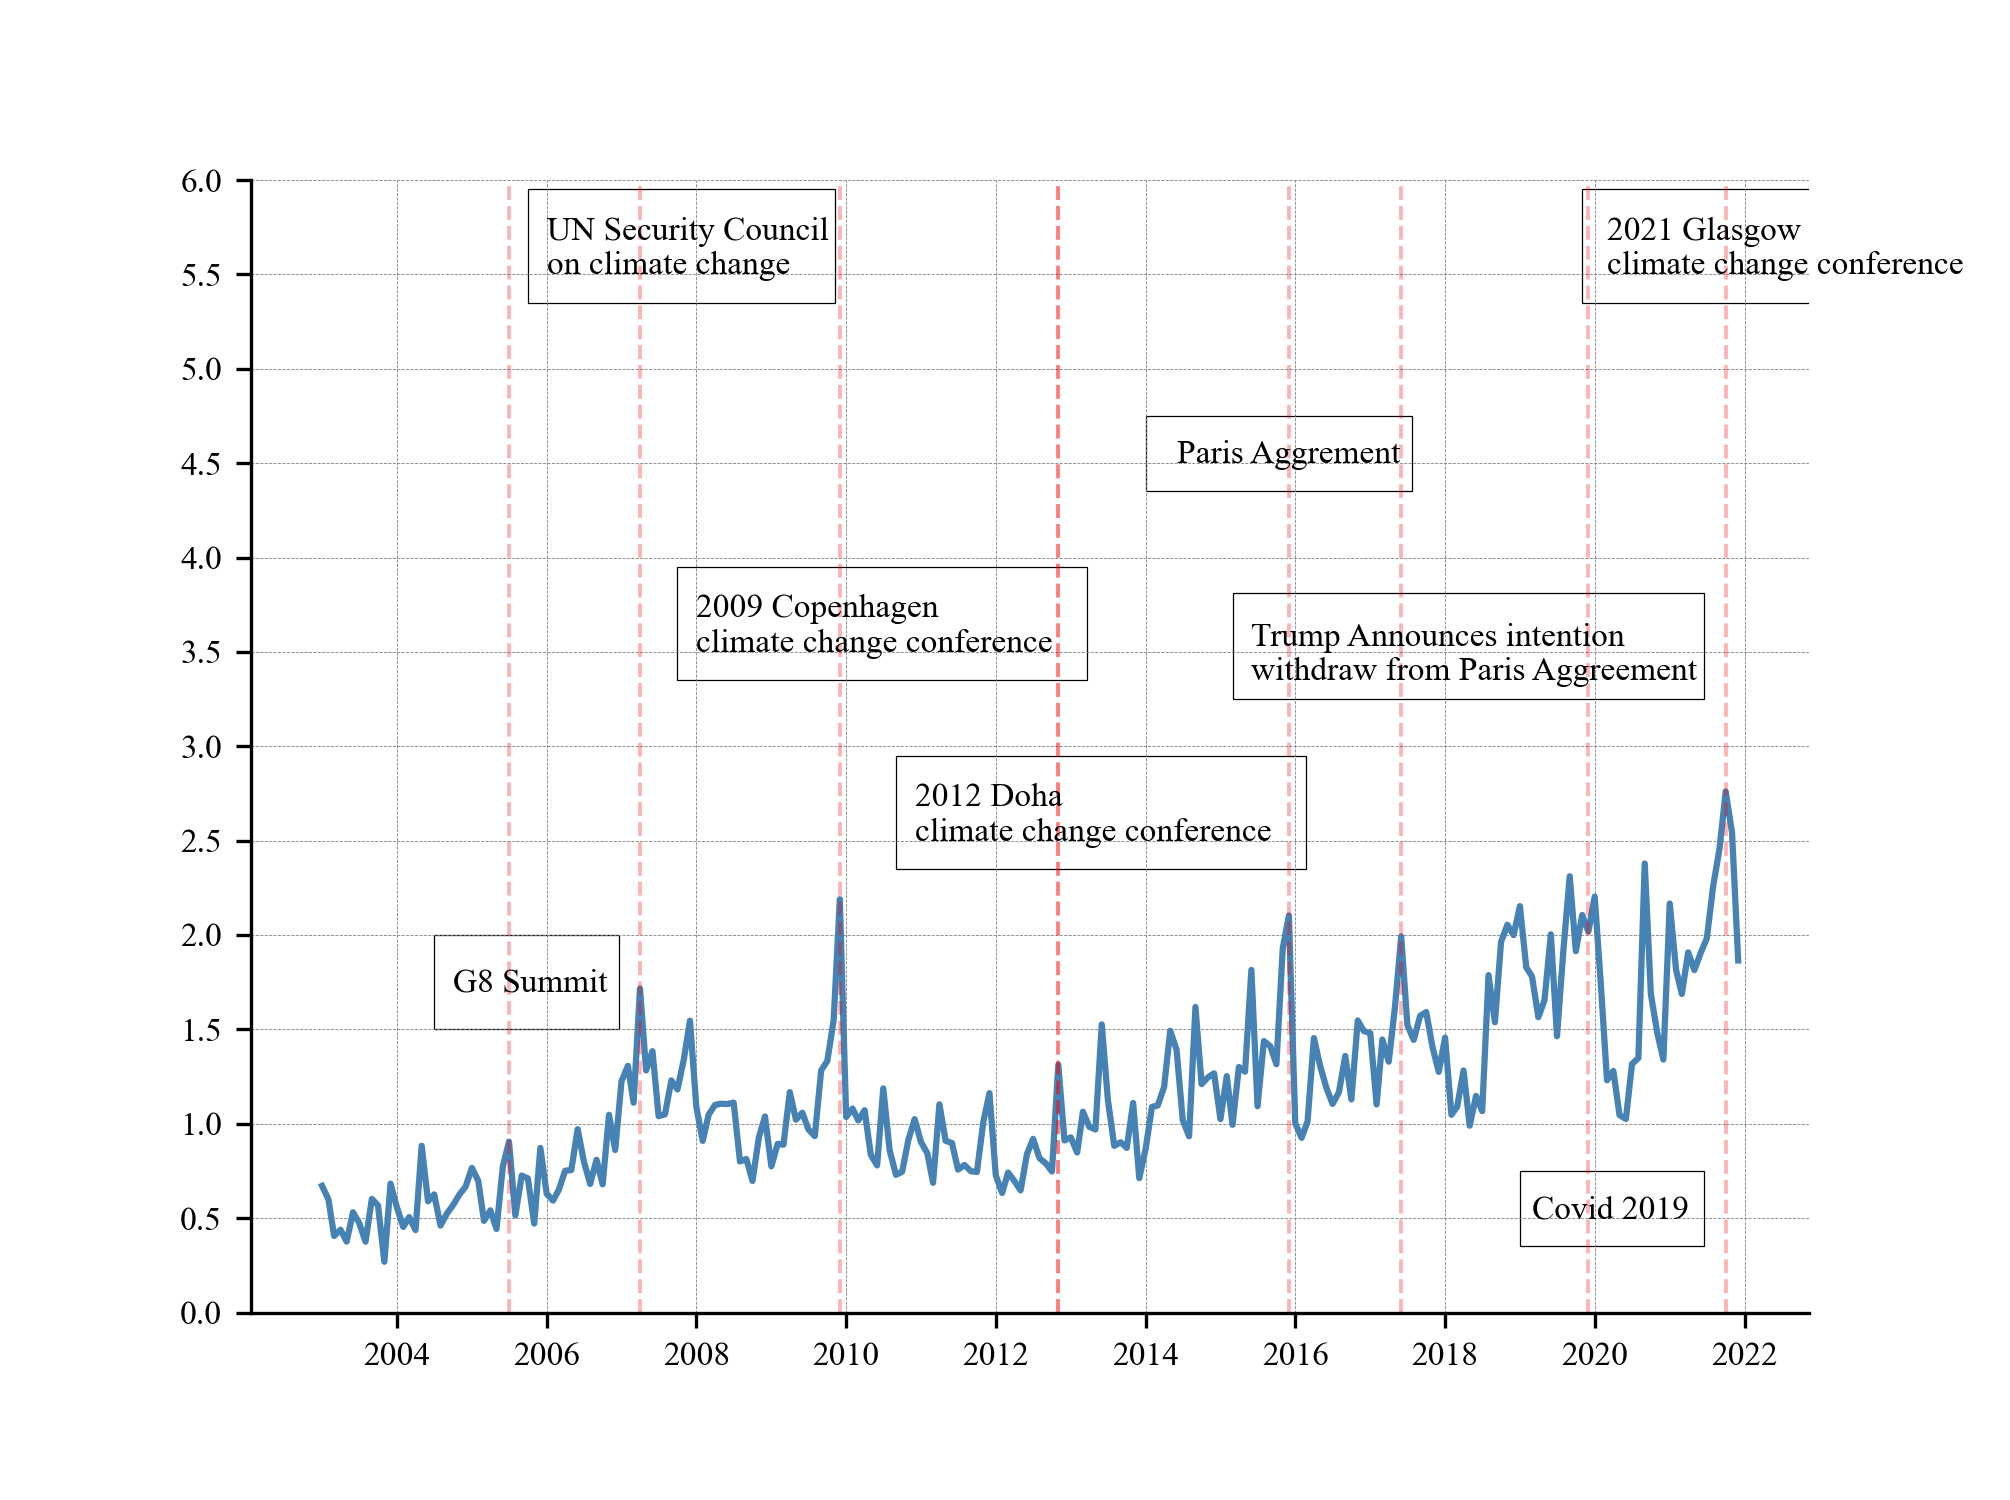
\includegraphics{graphics/mccc.png}
\label{fig: mccc}
\caption*{\footnotesize{This figure presents the monthly MCCC (Media Climate Change Concerns) index from 2003 to 2021 together with the major climate-related events.}}
\end{figure}
%%%%%%%%%%%%%%%%%%%%%%%%%%%%%%%%%%%%%%%%%%%%%%%%%%%
Presented in Table \ref{tab: on_umc}, the regression findings illuminate the outcomes of diverse portfolios structured based on firms' CO2 emissions in relation to the UMC index, accompanied by a set of control variables as specified by Equation \ref{eqn: test_pastor_model}. Upon examination, our initial observation surfaces: all portfolios, except for the Neutral portfolio\footnote{It's important to clarify that the neutral portfolio does not signify null CO2 emissions. Instead, firms within this portfolio exhibit total carbon emissions ranging between the 34th and 66th percentiles across the entire sample.}, showcase statistically insignificant intercepts. This suggests that the incorporation of the UMC index adeptly explains the returns across all portfolios. In the first column, notable trends emerge. The Green-Brown portfolio reveals its potential to accrue an average increase of 1.39\% in returns with each unit augmentation in the UMC index. This effect holds significant at the 1\% level. Contrarily, the third column captures the Brown portfolio's response, indicating an average decrease of -1.27\% in returns per unit uptick in the UMC index. Intriguingly, the UMC coefficient for the Neutral portfolio fails to achieve significance, indicating that the UMC index does not have a marginal influence on its returns. Lastly, in the second column, while a positive correlation between the Green portfolio and the UMC index aligns with our expectations, unfortunately, we do not observe significant statistical evidence to support our hypothesis.

%%%%%%%%%%%%%%%%%%%%%%%%%%%%%%%%%%%%%%%%%%%%%%%%%%%
\begin{table}[H]
\centering
\footnotesize
\caption{Green - Brown on UMC}
\label{tab: on_umc}
{
\def\sym#1{\ifmmode^{#1}\else\(^{#1}\)\fi}
\begin{tabular}{@{\extracolsep{2pt}}l*{4}{c}@{}}
\toprule
& \multicolumn{4}{c}{Dependent Variable}\\
\cline{2-5}
               & Green-Brown & Green    & Brown     & Neutral   \\
\hline
Intercept      & 1.310       & 1.665**  & 0.355     & 1.040**   \\
               & (1.179)     & (0.844)  & (0.857)   & (0.430)   \\
UMC            & 3.049***    & 1.786**  & -1.263*   & -0.029    \\
               & (1.029)     & (0.736)  & (0.748)   & (0.375)   \\
Mkt\_RF        & 0.083       & 0.920*** & 0.837***  & 0.965***  \\
               & (0.080)     & (0.057)  & (0.058)   & (0.029)   \\
SMB            & 1.079***    & 0.724*** & -0.355*** & 0.318***  \\
               & (0.133)     & (0.095)  & (0.096)   & (0.048)   \\
HML            & -0.557***   & -0.216** & 0.341***  & -0.008    \\
               & (0.122)     & (0.088)  & (0.089)   & (0.045)   \\
RMW            & -0.164      & -0.198*  & -0.033    & -0.024    \\
               & (0.167)     & (0.119)  & (0.121)   & (0.061)   \\
CMA            & 0.112       & 0.041    & -0.070    & -0.145*   \\
               & (0.208)     & (0.149)  & (0.151)   & (0.076)   \\
SENT           & 1.277**     & 0.971**  & -0.306    & 0.072     \\
               & (0.611)     & (0.437)  & (0.444)   & (0.223)   \\
WTI            & -0.010      & -0.014*  & -0.005    & -0.006    \\
               & (0.012)     & (0.009)  & (0.009)   & (0.004)   \\
CFNAI          & -0.046      & 0.121    & 0.167     & -0.016    \\
               & (0.200)     & (0.143)  & (0.145)   & (0.073)   \\
VIX            & 0.037       & 0.062**  & 0.025     & 0.016     \\
               & (0.040)     & (0.028)  & (0.029)   & (0.014)   \\

\hline
Obs & 227 & 227 & 227 & 227 \\
R-squared      & 0.368       & 0.742    & 0.590     & 0.903     \\
\bottomrule
\multicolumn{5}{l}{\footnotesize * p\sym{<}.1, ** p\sym{<}.05, *** p\sym{<}.01}
\end{tabular}
}
\begin{tablenotes}
    \item This table represents the regression results of Green-Brown, Green, Brown, and Neutral portfolios on the UMC index and a group of control variables. \citet{ardia2022climate} constructed the MCCC index since January 2003, hence the number of observations is less than 240. The Green Portfolio contains firms with total CO2 emissions up to the 33rd percentile, Neutral Portfolio contains firms with total CO2 emissions ranging from the 34th to 66th percentile, and firms with CO2 emissions higher than the 66th percentile are included in the Brown Portfolio. Green-Brown Portfolio is the monthly difference between Green and Brown portfolios.
\end{tablenotes}
\end{table}
%%%%%%%%%%%%%%%%%%%%%%%%%%%%%%%%%%%%%%%%%%%%%%%%%%%
\subsection{Firm Level Evidence}

In the previous section, we constructed Green and Brown portfolios based on firms' total carbon emissions. Interestingly, our findings showcased the Green portfolio's consistent outperformance over the Brown portfolio, particularly in the presence of high unexpected climate concerns (UMC). This trend appears to diverge from the conclusions drawn by \cite{bolton2021investors}, who, employing firm-level data, reveal a contrasting pattern. Their study highlights that firms characterized by higher carbon emissions (referred to as Brown firms in our context) tend to yield greater realized stock returns. Their interpretation centers around the integration of the climate risk premium within these returns. This notion indicates that investors factor in the associated climate risk, and require compensation from firms with higher climate risk exposure (firms with higher carbon emissions). As per their reasoning, elevated carbon emissions are linked with heightened climate risk, thus justifying the anticipation of a commensurately higher risk premium. In this section, we aim to critically revisit the empirical evidence from firm-level analysis.

To decipher the intricate relationship between companies' total CO2 emissions and their stock returns, we utilize a robust approach. We undertake the estimation of a time series regression model using Panel OLS:

\begin{equation}
    \label{eqn: firm_level}
    RET_{i,t} = \alpha + \beta_1 CO2\_tot_{i,t} + \beta_2 Contorls_{i,t} + \epsilon_{i,t}
\end{equation}

Here, $RET_{i,t}$ represents the stock return of firm $i$ during month $t$, and $CO2_{tot}$ corresponds to firms' total CO2 emissions, scaled logarithmically. The vector $Controls_{i,t}$ encompasses a range of control variables, encompassing firm-specific factors known for their predictive influence on returns. These variables include firm size (logged), leverage (total liability divided by total assets), B/M (book-to-market ratios), RoE (return on equity), Inves/AT (investment scaled by total assets), PPE (Property, plant, and equipment, logged), SaleGR (sales growth), EPS (earnings per share), Staff\_num (number of staff, logged), and Firm\_age (years since foundation). Our primary focus lies in interpreting the coefficient $\beta_1$, which plays a pivotal role in our investigation.

%%%%%%%%%%%%%%%%%%%%%%%%%%%%%%%%%%%%%%%%%%%%%%%%%%%
\subsubsection{Benchmark Result}

Based on Equation \ref{eqn: firm_level}, the findings are presented in Table \ref{tab: firm_level}, showcasing the results of firm-level analysis across two different fixed effects specifications for both the restricted and unrestricted models. In our approach, we use time-fixed effects at the month level. This choice serves to mitigate the impact of temporal variations across time, including broader economic conditions, shifts in investors' sentiments towards the stock market, the evolving concern for climate change, and other time-dependent factors. Columns 1 and 2 elucidate the outcomes of the regression analysis for the unrestricted and restricted models, respectively, incorporating Time + Industry two-way fixed effects. Notably, these techniques align with the methodologies employed by \cite{bolton2021investors}. By integrating industry-fixed effect, we effectively control for variations across distinct industries. This approach permits us to find the average correlation between firms' total CO2 emissions and stock return cross-sectionally without the influence to which industry a firm belongs. 

For the unrestricted model presented in column 1, we find a positive correlation between firms' total CO2 emissions and stock return, However, the near-zero R-squared value indicates limited explanatory power, potentially attributed to omitted variables. Moving to column 2, the restricted model's outcomes are showcased. The consistent positive relationship between firms' total CO2 emissions and stock returns persists but loses statistical significance. Different from \cite{bolton2021investors} paper, where they get significant results between stock return and various scopes of CO2 emissions by excluding firms from salient industries (GIC 19, 20, 23), here we analyze all the firms regardless of which industry they belong to. Furthermore, an additional consideration raised by \cite{aswani2023carbon} involves the potential for collinearity between firm size and CO2 emissions. They argue that the apparent positive link between CO2 emissions and stock returns might be influenced by this collinearity. There is no doubt that larger firms tend to have more CO2 emissions, and industry-level fixed effects can not identify this collinearity issue.

Columns 3 and 4 in Table \ref{tab: firm_level} showcase the un/-restricted model with Time + Entity (firm) two-way fixed effects. Different from Time + Industry two-way fixed effects, with Time + Entity fixed effects the analysis considers both time-specific variations and variations unique to individual entities (firms). By including Entity fixed effects, we are accounting for firm-specific factors that may be constant over time but vary across different firms. This is a more stringent restriction by the assumption that investors not only distinguish industry-specific characteristics but also place a heightened emphasis on each firm's specific inherent attributes. 

First, it is important to note that the results remain consistent between the un-/restricted models presented in columns 3 and 4. Then, the most intriguing revelation arises from the incorporation of Time + Entity two-way fixed effects, leading to an observed sign reversal of the coefficient on CO2 emissions. This shift takes place under the assumption that investors place greater emphasis on each firm's intrinsic attributes rather than industry-specific characteristics. Specifically, firms with higher CO2 emissions, implying increased exposure to climate risks, tend to exhibit lower stock returns on average. Importantly, this observation maintains both economic and statistical significance. And it's important to underscore that this finding aligns with the persistent outperformance of the Green portfolio over the Brown portfolio. Finally, given that the positive relationship between firm size and stock returns persists, concerns of collinearity between CO2 emissions and firm size in predicting stock returns, as brought up by \cite{aswani2023carbon} are no longer applicable.\footnote{Table \ref{tab: corr} shows there is a positive correlation between firms' CO2 emissions and their size, but the relationship between return and CO2 emissions has an opposite sign to the relationship between return and size.}


\begin{table}[H]
\centering
\footnotesize
\caption{Firm Level Analysis}
\label{tab: firm_level}
{
\def\sym#1{\ifmmode^{#1}\else\(^{#1}\)\fi}
\begin{tabular}{@{\extracolsep{2pt}}l*{4}{c}@{}}
\toprule
& \multicolumn{4}{c}{Returns} \\
\cline{2-5}
 & (1) & (2) & (3) & (4) \\
\hline
CO2\_tot & 0.075\sym{*} & 0.034 & -0.176\sym{**} & -0.659\sym{***} \\
 & (0.040) & (0.053) & (0.090) & (0.127) \\
Size &  & 0.250\sym{**} &  & 1.535\sym{***} \\
 &  & (0.101) &  & (0.197) \\
Levarage &  & -0.226 &  & 0.173 \\
 &  & (0.203) &  & (0.422) \\
B/M &  & -1.879\sym{***} &  & -2.729\sym{***} \\
 &  & (0.181) &  & (0.276) \\
RoE &  & 0.526\sym{***} &  & 0.292\sym{***} \\
 &  & (0.086) &  & (0.101) \\
Inves/AT &  & -4.447\sym{***} &  & -12.650\sym{***} \\
 &  & (1.132) &  & (1.874) \\
PPE &  & -0.008 &  & -0.426\sym{***} \\
 &  & (0.048) &  & (0.162) \\
SaleGR &  & 0.916\sym{***} &  & 0.799\sym{***} \\
 &  & (0.224) &  & (0.237) \\
EPS &  & 0.057\sym{***} &  & 0.018 \\
 &  & (0.022) &  & (0.027) \\
Staff\_num &  & -0.278\sym{***} &  & -0.835\sym{***} \\
 &  & (0.066) &  & (0.213) \\
Firm\_age &  & -0.047 &  & 1.789\sym{***} \\
 &  & (0.065) &  & (0.517) \\
Constant & 0.162 & 0.526 & 3.353\sym{***} & -3.421 \\
 & (0.505) & (0.643) & (1.137) & (2.940) \\

\hline
Firm F.E. & No & No & Yes & Yes \\
Industry F.E. & Yes & Yes & No & No \\
Year-Month F.E. & Yes & Yes & Yes & Yes \\
\hline
Obs & 466999 & 295704 & 466999 & 295704 \\
R-squared & 0.000 & 0.013 & 0.000 & 0.019 \\
\bottomrule
\multicolumn{5}{l}{\footnotesize * p\sym{<}.1, ** p\sym{<}.05, *** p\sym{<}.01}
\end{tabular}
}
\begin{tablenotes}
    \item This table presents the regression results depicting the influence of firms' CO2 emissions on stock returns. To account for potential dependencies within the data, the standard errors are clustered at the specified level along with the fixed effects integrated into the model.
\end{tablenotes}
\end{table}

%%%%%%%%%%%%%%%%%%%%%%%%%%%%%%%%%%%%%%%%%%%%%%%%%%%
\subsubsection{Robustness Check}

In the context of the regression model \ref{eqn: firm_level}, the choice of fixed effects can vary depending on the underlying assumptions. In conventional cross-sectional stock return analyses, it is a common practice to assume significant heterogeneity between industries, with the belief that firms within a particular industry exhibit similar characteristics in terms of their stock returns. This assumption has garnered substantial empirical support in the existing literature. However, it's crucial to recognize that investors base their investment allocation decisions on more than just industry categorizations. While they may initially screen industries, their ultimate investment choices often depend on the specific attributes of individual companies. In such scenarios, even firms within the same industry can exhibit significant variations in their stock performance. Therefore, considering heterogeneity at the firm level may be a more suitable approach than relying solely on industry-level assumptions. In the following analysis, we perform a robustness check with various fixed effects and cluster standard errors at different levels.

The first six models depicted in Figure \ref{fig: forestplot} include the benchmark model along with variations involving different fixed effects. In the case of considering only the Entity fixed effect, we observe a coefficient of -0.74 for total CO2 emissions, which is statistically significant at the 1\% level. Similarly, when we incorporate both Entity and Year two-way fixed effects, the CO2 emissions coefficient remains statistically significant at the 1\% level, with a slightly reduced value of -0.72. These specifications maintain consistency with the benchmark model, showing only minor coefficient adjustments. Moving on to models 4, 5, and 6, where we introduce industry fixed effects, industry + year-month, and industry + year two-way fixed effects, we observe a different pattern. In these models, the coefficients on CO2 emissions all become statistically insignificant and approach zero.

\cite{white1980heteroskedasticity} in his seminar paper first introduced Robust standard errors in econometrics to account for heteroscedasticity. In Model \ref{eqn: firm_level}, which retains the same fixed effects as the benchmark model, the application of robust standard errors significantly increases statistical significance and narrows down the confidence intervals as depicted by the 7th model in Figure \ref{fig: forestplot}. Furthermore, as highlighted by \cite{petersen2008estimating}, in corporate and empirical and asset pricing research, when dealing with panel data the residuals may be correlated across firms or across time. In such cases, standard errors can be biased. To mitigate this, Petersen recommends clustering standard errors at the same level, as is done in our benchmark model. Additionally, \cite{angrist2009mostly} advocates for clustering standard errors at a level one step above the sample data. In line with this recommendation, we cluster the standard errors at the industry and year level for the benchmark model to test its robustness. After applying clustering to standard errors at the Industry + Year level, we observe a slight increase in standard errors compared to the benchmark model. Nonetheless, the results remain statistically significant at the 1\% level, as shown by the last model in Figure \ref{fig: forestplot}.

%%%%%%%%%%%%%%%%%%%%%%%%%%%%%%%%%%%%%%%%%%%%%%%%%%%
\begin{figure}[H]
\centering
\caption{\textbf{Change of Fixed Effects and Cluster Levels}}
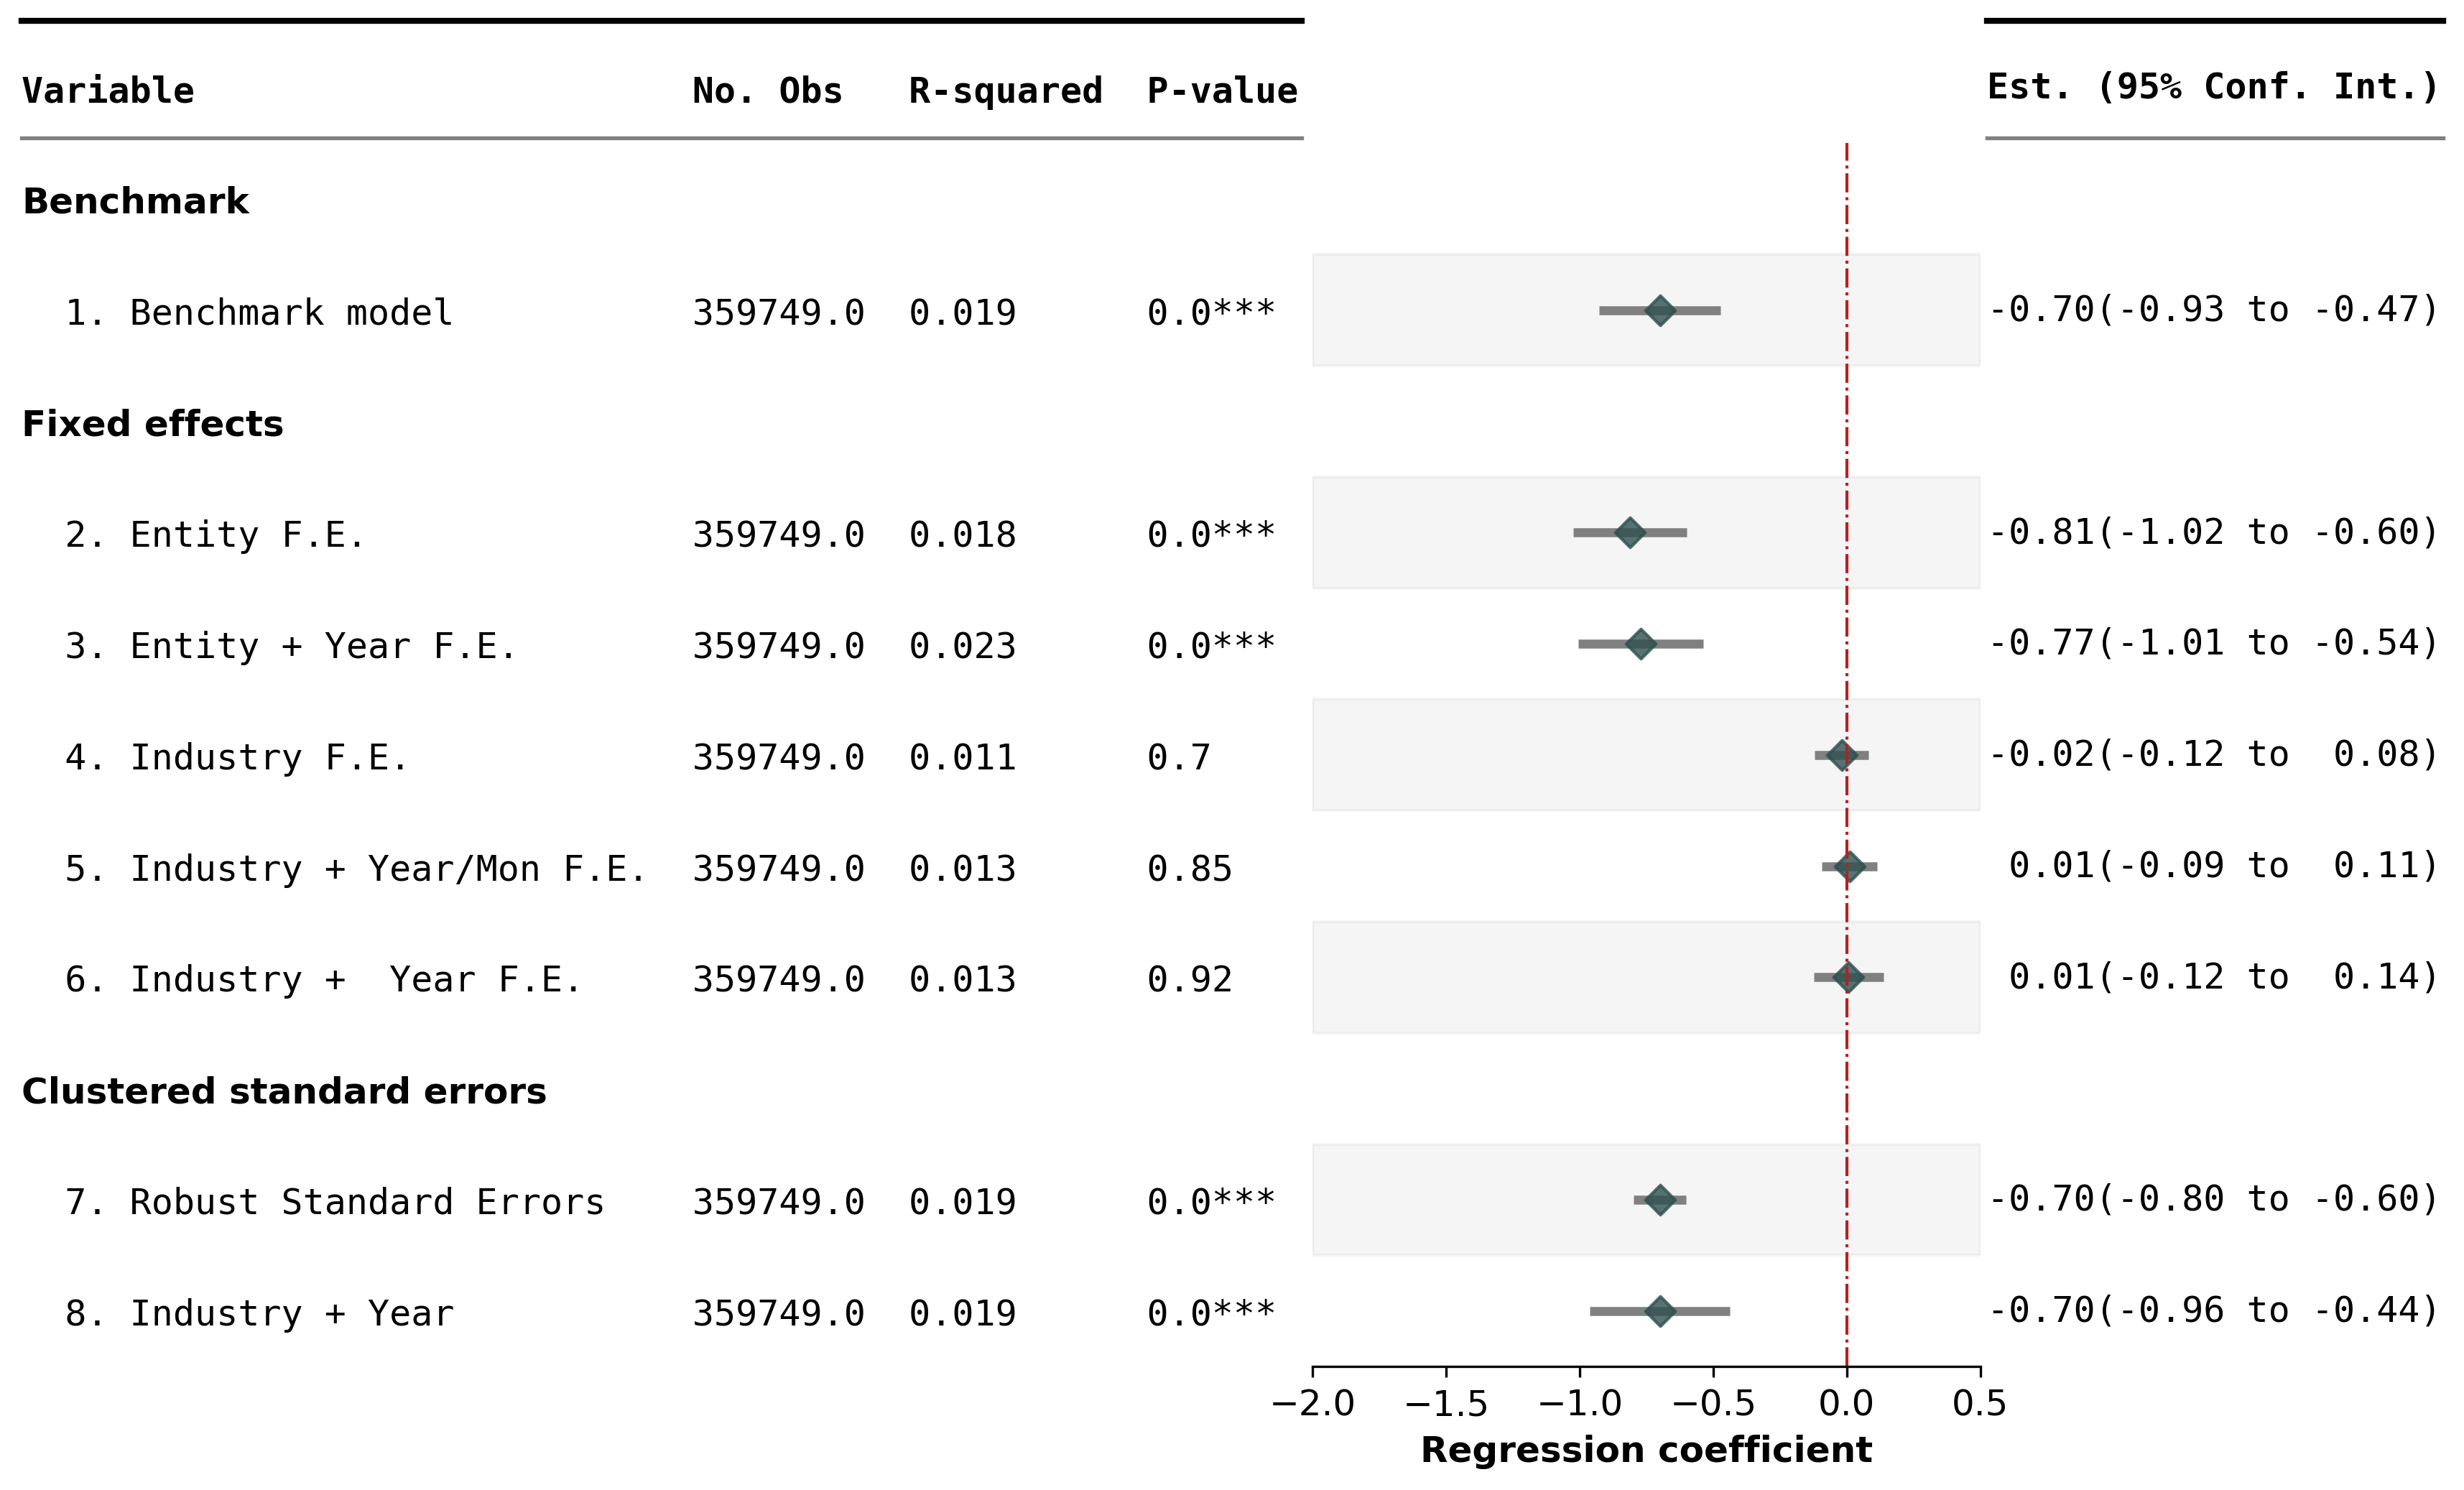
\includegraphics[width=.8\textwidth]{graphics/forestplot.png}
\label{fig: forestplot}
\caption*{\footnotesize{This graphic presents coefficients and associated confidence intervals for various fixed effects and clustered standard error configurations. The benchmark model includes Entity + Year/Month fixed effects, with standard errors clustered at the same level. In the 'Fixed Effects' group, we explore different fixed effects for each model, while maintaining standard errors clustered at the same level. In the 'Clustered Standard Errors' group, we examine how standard errors are clustered at various levels while keeping the fixed effects consistent with the benchmark model.}}
\end{figure}

%%%%%%%%%%%%%%%%%%%%%%%%%%%%%%%%%%%%%%%%%%%%%%%%%%%
\subsubsection{Interplay with climate concerns}
In the previous section, we find a negative relationship between firms' CO2 emissions and their stock returns when using Time + Entity two-way fixed effects. This finding holds true under the assumption that investors not only differentiate between industry-specific characteristics but also place significant emphasis on the unique characteristics of each firm. The reason behind this relationship may be linked to investors' growing commitment to green investing mandates and their increasing concerns about the potential risks posed by climate change. Consequently, it becomes intriguing to delve into the dynamic between a firm's CO2 emissions and public climate concerns. One plausible hypothesis is that during periods of elevated climate concern, firms with higher CO2 emissions (i.e., more environmentally polluting firms) tend to experience lower stock returns. This conjecture aligns with the research by \cite{gabaix2021search}, which suggests that the price elasticity of demand in the aggregate stock market is relatively small, and significant flows of capital in and out of the stock market can exert substantial influence on prices. Similar insights were offered by \cite{koijen2019demand}, indicating that if investors divest from assets associated with such firms, it could lead to a drop in their stock returns.

To investigate the relationship between firms' carbon emissions, public climate concerns, and their stock returns, we propose a firm fixed-effect panel regression model, as expressed in Equation \ref{eqn: firm_co2}:

\begin{equation}
\label{eqn: firm_co2}
\begin{aligned}
RET_{i,t} = & \alpha + \beta_1 CO2\_tot_{i, t} + \beta_2 UMC_{t} + \beta_3 interaction_{i,t} &+ \\
            & \beta_4 Time Variates_t + \beta_5 Controls_{i, t} + \epsilon_{i, t}
\end{aligned}
\end{equation}

In this model, $Co2\_tot_{i,t}$ represents firm $i's$ total carbon mission in month $t$,  $UMC_t$ represents monthly unexpected media climate concerns at month $t$. $UMC$ index is a variable that is updated monthly and serves as a focal point in our regression analysis. Given its frequent updates, we refrain from using a time-fixed effect to absorb its effects on our dependent variable. $interaction_{i,t}$ is the interaction between $Co2\_tot_{i,t}$ and $UMC$. To account for other time-related variations, we incorporate $Time Variates_t$, which could encompass variables such as FF-3 factors to capture market information, sentiment indicators to gauge investor sentiment, the VIX to measure market trading volatility, and other relevant factors. Additionally, $Controls_{i,t}$ represents a vector of firm-specific characteristic variables, such as size, leverage, and more, which are relevant to our analysis.


\begin{table}[H]
\centering
\footnotesize
\caption{Cross-section Stock Return with UMC}
\label{tab: firm_umc}
{
\def\sym#1{\ifmmode^{#1}\else\(^{#1}\)\fi}
\begin{tabular}{@{\extracolsep{2pt}}l*{4}{c}@{}}
\toprule

& \multicolumn{4}{c}{Dependent variable: Return} \\
\cline{2-5}
 & (1) & (2) & (3) & (4) \\
\hline
CO2\_tot & -0.569\sym{***} & -0.580\sym{***} & -0.580\sym{***} & -0.578\sym{***} \\
 & (0.112) & (0.109) & (0.109) & (0.111) \\
UMC & 1.648\sym{***} & 1.688\sym{***} & 1.460\sym{***} & 1.749\sym{***} \\
 & (0.402) & (0.401) & (0.403) & (0.405) \\
interaction & -0.135\sym{***} & -0.145\sym{***} & -0.133\sym{***} & -0.150\sym{***} \\
 & (0.029) & (0.028) & (0.029) & (0.029) \\
Mkt\_RF & 0.999\sym{***} & 0.909\sym{***} & 0.915\sym{***} & 0.949\sym{***} \\
 & (0.010) & (0.009) & (0.008) & (0.009) \\
SMB &  & 0.383\sym{***} & 0.360\sym{***} & 0.321\sym{***} \\
 &  & (0.013) & (0.013) & (0.013) \\
HML &  & 0.012 & 0.002 & 0.046\sym{***} \\
 &  & (0.010) & (0.010) & (0.010) \\
RMW &  &  & -0.065\sym{***} & -0.042\sym{***} \\
 &  &  & (0.014) & (0.015) \\
CMA &  &  & 0.063\sym{***} & 0.048\sym{***} \\
 &  &  & (0.016) & (0.016) \\
SENT &  &  &  & -0.497\sym{***} \\
 &  &  &  & (0.042) \\
WTI &  &  &  & -0.009\sym{***} \\
 &  &  &  & (0.001) \\
CFNAI &  &  &  & 0.012 \\
 &  &  &  & (0.013) \\
VIX &  &  &  & 0.047\sym{***} \\
 &  &  &  & (0.003) \\
Constant & 1.828 & 1.100 & 0.992 & -0.911 \\
 & (1.915) & (1.940) & (1.946) & (1.936) \\

\hline
Controls & Yes & Yes & Yes & Yes \\
Entity F.E. & Yes & Yes & Yes & Yes \\
Obs & 295215 & 295215 & 295215 & 295215 \\
R-squared & 0.203 & 0.212 & 0.213 & 0.215 \\
\bottomrule
\multicolumn{5}{l}{\footnotesize * p\sym{<}.1, ** p\sym{<}.05, *** p\sym{<}.01}
\end{tabular}
}
\end{table}

In the context of Equation \ref{eqn: firm_co2}, we anticipate the coefficient $\beta_1$ to be notably negative, as previously demonstrated in our analysis. However, the interpretation of $\beta_2$ remains less straightforward. Our earlier findings, as presented in Table \ref{tab: on_umc}, indicate that a higher $UMC$ value favors Green rather than Brown portfolios. Consequently, the overall impact of $UMC$ on stock returns across the entire sample remains somewhat uncertain. Nonetheless, the most focused coefficient within this specification is $\beta_3$ representing the interaction term between $CO2\_tot_{i,t}$ and $UMC_t$. Our expectation is a negative value for $\beta_3$ suggesting that when unexpected climate concerns are high, firms with higher total CO2 emissions are likely to experience lower stock returns. This hypothesis aligns with our belief that increased climate concern prompts a negative market response for environmentally intensive firms.

Table \ref{tab: firm_umc} presents the regression results for Model \ref{eqn: firm_co2}, with standard errors clustered at the entity level. Regardless of the various controls included in $TimeVariates_{i,t}$, a consistent pattern emerges in the results. The coefficient on $CO2\_tot_{i,t}$ consistently exhibits a statistically significant negative relationship with stock returns, aligning with the findings presented in Table \ref{tab: firm_level}. Furthermore, the coefficient on $UMC_t$ consistently appears positive, indicating that, on average, higher unexpected climate concern is associated with higher stock returns. Lastly, the coefficient on $interaction_{i,t}$ consistently appears negative, regardless of the controls used. This suggests that when unexpected climate concern is elevated, the stock returns of Brown firms, characterized by higher total CO2 emissions, tend to decline on average, and the statistical significance holds at 1\% level.

\clearpage
%%%%%%%%%%%%%%%%%%%%%%%%%%%%%%%%%%%%%%%%%%%%%%%%%%%%%%%%%%%%%%%%
%%%%%%%%%%%%%%%%%%%%%%%%%%%%%%%%%%%%%%%%%%%%%%%%%%%%%%%%%%%%%%%%
\section{Conclusion} \label{sec:conclusion}
%%%%%%%%%%%%%%%%%%%%%%%%%%%%%%%%%%%%%%%%%%%%%%%%%%%%%%%

This paper seeks to unravel a paradox that has emerged in recent years in the realm of sustainable investing. On one hand, the aggregate performance of Green portfolios, composed of companies with lower carbon emissions or higher ESG (Environmental, Social, and Governance) scores, has exhibited a consistent and noteworthy outperformance compared to their Brown counterparts. This phenomenon is commonly referred to as the "green premium" and is attributed to the increasing concerns surrounding climate change and environmental sustainability. It reflects a growing trend among investors who are increasingly inclined to allocate capital to assets that align with sustainable and environmentally responsible practices.

However, when we shift our focus to the firm-level empirical analysis, a seemingly contradictory picture emerges. Here, the data often presents a different narrative, one where Brown firms, those associated with higher carbon footprints or lower ESG scores, appear to yield higher expected stock returns. This observation challenges the conventional wisdom of sustainable investing and introduces the notion of a "climate risk premium." Investors seem to be demanding higher returns as compensation for investing in companies with perceived sustainability and climate-related risks.

The existence of this paradox raises crucial questions and calls for a deeper examination. Why do Green portfolios, at the aggregate level, consistently outperform their Brown counterparts when firm-level data suggests otherwise? Is the green premium truly a reflection of superior financial performance, or are there underlying factors that need to be considered? Moreover, what explains the climate risk premium observed at the firm level, and how do these findings align with the broader goals of sustainable and responsible investing?

This paper embarks on a comprehensive journey to dissect these questions and shed light on the complex and evolving landscape of sustainable investing. By conducting rigorous analyses that combine cross-sectional evidence, portfolio performance assessments, and firm-level empirical investigations, we find that, under different assumptions with varying model specifications, firm-level results coincide with aggregate portfolio analysis. Specifically, Brown firms with higher carbon footprints are more exposed to climate change-related risks and tend to underperform Green firms with lower carbon footprints in terms of stock returns, particularly when there are heightened concerns about unexpected climate change. Through these endeavors, we aim to provide valuable insights that can inform investment decisions, drive sustainable practices, and contribute to a more nuanced understanding of the relationship between sustainability and financial returns in the context of our ever-changing global landscape.
\clearpage
%%%%%%%%%%%%%%%%%%%%%%%%%%%%%%%%%%%%%%%%%%%%%%%%%%%%%%%%%%%%%%%%
%%%%%%%%%%%%%%%%%%%%%%%%%%%%%%%%%%%%%%%%%%%%%%%%%%%%%%%%%%%%%%%%
\begingroup
\setstretch{1.0}
\bibliographystyle{plainnat}
\bibliography{citation}
\endgroup

\clearpage
%%%%%%%%%%%%%%%%%%%%%%%%%%%%%%%%%%%%%%%%%%%%%%%%%%%%%%%%%%%%%%%%
%%%%%%%%%%%%%%%%%%%%%%%%  Appendix  %%%%%%%%%%%%%%%%%%%%%%%%%%%%
%%%%%%%%%%%%%%%%%%%%%%%%%%%%%%%%%%%%%%%%%%%%%%%%%%%%%%%%%%%%%%%%
% By default figure number is continuous on appendix. You can change this by the following two lines
%\setcounter{figure}{0}
%\setcounter{table}{0}
%\renewcommand\thetable{\Alph{section}.\arabic{table}}
%\renewcommand\thefigure{\Alph{section}.\arabic{figure}}

%\section*{Appendix A} \label{sec: appendixa}
%\addcontentsline{toc}{section}{Appendix A}
%\subsection{Average Monthly Return on Other Indicators}
\end{document}
